\documentclass[a4paper,11pt]{report}
%\usepackage{hyperref}
\usepackage{url,natbib,amssymb,hyperref,graphicx,wrapfig,setspace,multirow,booktabs,subfig,array,wrapfig,calc}
\usepackage{array}
\newcolumntype{P}[1]{>{\centering\arraybackslash}p{#1}}
\usepackage{fancyhdr}
\usepackage{color}
\usepackage{booktabs,caption,fixltx2e}
\usepackage[round]{natbib}      % References with names and years
\usepackage{xr}                 % reference anothe chapter
%\externaldocument[2-]{../CHAPTER2/ch2_LSM_v11}
%\externaldocument[3-]{../CHAPTER3/ch3_sensitivity_v10}
\usepackage{graphicx}
\usepackage{caption}
\usepackage{appendix}
%\usepackage{subfigure}
\usepackage{float}
\usepackage{subfig}
\usepackage{float}
\usepackage{paralist}                % inline lists
\usepackage{gensymb}    % degrees celsius as {\celsius}
%\usepackage{textcomp]    % arrows
\newcommand{\tildetext}{\raise.17ex\hbox{$\scriptstyle\mattt{\sim}$}}
\usepackage{rotating}   %rotate table
%\renewcommand{\arraystretch}{1.5}  %increase space between rows in tables (default is 1) because there is already baselinestrech 1.5 tables become too separated, maybe with normal spacing this command should be used
\usepackage{rotating,booktabs}
\usepackage{threeparttable}
\usepackage{multirow}
\usepackage{color}% color the text
\usepackage{amsmath}
% Page setup from thesis template
\topmargin=-10mm
\textwidth=150mm
\textheight=234mm
\headsep=12mm
\oddsidemargin=14mm
%\oddsidemargin=12mm
\evensidemargin=-1mm
%\evensidemargin=1mm
\parindent=6mm
\parskip=1em 

\newlength{\rulewidth}
\setlength{\rulewidth}{150mm} % change to 150mm for printing on
			      % gordon, 149 otherwise???
% 1.5 line spacing so my supervisor can scrawl all over it
\renewcommand{\baselinestretch}{1.50}

\pagestyle{headings}    % chapter number on top

\setcounter{secnumdepth}{4}              %Numbers subsubsections, and lower.
\setcounter{tocdepth}{4}                 %Sets depth of table of contents to include subsubsections.

\pagestyle{fancy}
\fancyhf{}
%\rhead{\fancyplain{}{\textit{\nouppercase\rightmark}}}
\fancyhead[L]{\textit{Chapter 4: Vegetation structure in Radiative Transfer schemes}}
\fancyfoot[C]{ \thepage\ }

%opening
\title{}
\author{Renato Kerches Braghiere \\ This document was written in \LaTeX \\ Number of words: 18135}
\date{\today}

\begin{document}
\maketitle
\setcounter{chapter}{3} %so next one is 4

\tableofcontents
\listoffigures
\listoftables

\chapter{Vegetation structure in Radiative Transfer schemes}
This chapter will discuss the impacts of vegetation canopy structure on shortwave radiation partitioning on its three components: absorption, reflectance and transmittance. It will introduce a novel perspective on how to account for vegetation structural effects on turbid media 1D radiative transfer schemes commonly used in weather forecast and climate predictions models by using an additional `effective factor'. The theory discussed before was already explored by several authors through many perspectives, but in here, these different parameterisations will be explored in order to determine pros and cons of each one of them and point out to whether or not to apply them. The main purpose of this chapter is to give to the reader a background knowledge through the performance of different experiments to ensure the limitations of 1D radiative transfer schemes when compared to more complex ones, and to address the ability of a simple parameterisation in reproduce the radiation partitioning of 3D radiative transfer schemes both zenithal and vertically.

\section{The effects of different vegetation canopy arrangements on PAR partitioning}
In this section a sensitivity analysis of radiation partitioning due to multiple canopy features is described. It is well documented in the literature that vegetation canopy structure affects the amount of radiation absorbed by plants, transmitted to the background soil and reflected back to the atmosphere, and it can have further impacts on the surface radiative balance and biogeophysical processes, as photosynthesis. However, only few studies looked at the impact of specific vegetation structural features on radiation partitioning or related variables.

\citet{Chen2008} performed a sensitivity analysis of clumping index ($\Omega$) \citep{Nilson1971,chen1992} with the MAESPA model \citep{Duursma2012} by changing vegetation canopy structural variables, as tree spacing, crown width and depth, leaf area density, the leaf angle distribution function and illumination conditions, as solar zenith angle. The authors found that solar zenith angle has a large impact on clumping that is highly dependent on tree spacing to crown width ratio ($l^{\prime}$), which determines whether or not trees cast shade each other. For very small $l^{\prime}$ ($\sim$10$^{-5}$) the vegetation canopy is comparable to the continuous case and the clumping factor is approximately 1. As soon as the tree spacing increases, the mutual shadowing starts to play an important role on the behaviour of clumping index with solar zenith angle. 

Different patterns indicate that the clumping index increases with solar zenith angle only in certain conditions. However, looking at clumping index alone does not tell much about how the radiation partitioning changes with different vegetation canopy structural features.

\subsection{Using 3D models to address the impacts of canopy structure on PAR partitioning}
To address the radiative transfer process in heterogeneous vegetation, the Geometric Optical Radiative Transfer (GORT) model conceptually combines geometric optical principles for canopy structure and radiative transfer theory for volumetric scattering within canopy crowns \citep{Li1995} and it is suitable to explore the impacts of structural effects on radiation partitioning. These effects come mainly from the fact that tree crowns cast shadows on one another and on the background soil, resulting in self-shadowing effects as described by the geometric-optical theory \citep{Li1992}. The GORT model was originally developed to model the bidirectional reflectance of discontinuous plant canopies \citep{Li1995}, it was then modified for modelling the solar radiation transmission and absorption by canopy elements. \citet{Ni1997} found that GORT modelled well the hierarchical clumping structure of plant canopies, including the clumping of needles into shoots, shoots into branches, branches into whorls, and whorls into crowns for conifer forests. The variables in GORT are distribution functions of tree geometry parameters such as mean tree size and density of a predefined ellipsoidal shape, and also the spectral properties of canopy elements and background. 

GORT models tree crowns as a collection of ellipsoids (Fig.~\ref{fig:gort_scheme}), of which the centres are randomly distributed between the upper and lower boundaries of the canopy layer ($h_1$ and $h_2$). Each ellipsoid, or each canopy crown, is characterised by one-half of the vertical crown length ($b$) and a horizontal crown radius ($R$). The total gap probability (P$_{gap}$) is modelled separately as the proportion of sunlight passing through the canopy layer without reaching any crown (hereafter referred to as between-crown gaps) and the proportion of sunlight passing through crowns without being intercepted by canopy leaves (hereafter referred to as within-crown gaps). 

\begin{figure}[ht]
      	\centering
        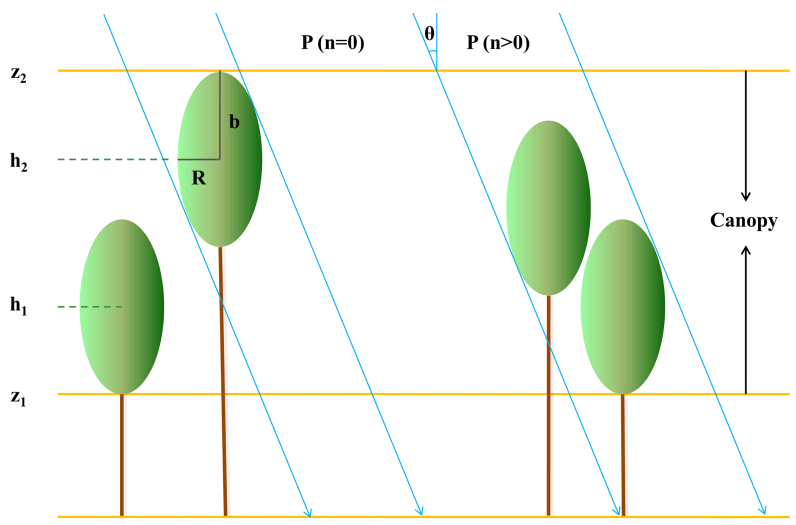
\includegraphics[width=0.5\textwidth]{/home/mn811042/Thesis/chapter4/figures/GORT_schematic.png}
        \caption{A scheme of the canopy structure in the Geometric Optical Radiative Transfer model as modified from \citet{Ni1998}.} 
\label{fig:gort_scheme}
\end{figure}

Gap probability, or direct transmissivity, is the probability of photons reaching a given vegetation canopy depth without being intercepted by plant elements. It is a key variable to characterise the radiation partitioning within vegetation canopies. A detailed description for modelling the gap probability with GORT is described in previous studies \citep{Li1995,Ni1999}. In here the concept of gap probability is briefly summarised. For  homogeneous  canopies,  Beer\textsc{\char13}s  law  describes  the gap  probability  of  sunlight  penetration, while for discontinuous plant canopies, leaves are clumped within individual canopy crowns, creating an uneven distribution of gap probabilities for beam radiation.

The goal of this section is to: 
\begin{enumerate}
\item explore the differences in absorbance, reflectance and transmittance in the PAR spectrum (400 - 700 nm) related to a series of variables including: structural (lower and upper boundary of the crown centres, tree density, vertical and horizontal crown radius and their ratio), geometrical (crown shape, leaf angle distributions and solar zenith angle), spectral (leaf and soil albedo) and optical (leaf area index, analogous to the optical depth of a canopy); and 
\end{enumerate}

A default canopy with LAI = 1.0 m$^2$.m$^{-2}$ and canopy cover of 20\% was set for this exercise and it is described in details in Table~\ref{tab:parameters_gort}. For all evaluated variables, the other ones were fixed on a base value and they varied in a predefined range. Except for the case of vertical to horizontal crown radius ratio ($b/R$), where both radius varied together following the range between 10$^{-3}$ to 10$^2$.

\begin{threeparttable}
\centering
\caption{Base values and ranges for parameters used in GORT or MAESPA.}
%\begin{tabular*}{\textwidth}{ l@{\extracolsep{\fill}}*{4}{c}}
\begin{tabular}{lP{0.20\textwidth} lP{0.25\textwidth} lP{0.25\textwidth} lP{0.25\textwidth}}
%\begin{tabular}{\textwidth}{|p{\textwidth/4}|p{\textwidth/4}|p{\textwidth/4}|p{\textwidth/4}|}
%\begin{tabular*}
     \hline
     \hline
\textbf{Parameter}   & \textbf{Description} & \textbf{Base Value (Unit)} & \textbf{Range} \\
\noalign{\smallskip}\hline
$h_1$          & Lower boundary of the crown centres       & 7.0  (0.01) m & 0.01 - 49.9 \\
$h_2$          & Upper boundary of the crown centres       & 11.0  (50) m & 0.02 - 50.0 \\
$\lambda$         & Tree density                              & 40 trees/ha &  1 - 1000\\
$b$            & Vertical crown radius                     & 5 m & 0 - 50\\ 
$R$            & Horizontal crown radius                   & 5 m &  0 - 50\\
$b/R$           & Vertical to horizontal crown radius ratio & 1 & 10$^{-3}$ - 10$^2$\\
LAI            & Leaf Area Index                           & 1.0 m$^2$.m$^{-2}$ &  0.1 - 10.0\\
$\omega_l$ \\ ($\rho_{leaf} + \tau_{leaf}$)          & Leaf single scattering albedo             & 0.13 &  0.00 - 1.00\\
$\alpha_{soil}$  & Soil albedo                               & 0.12 & 0.00 - 1.00\\ 
Shape$^*$           & Crown shape                               & Round & Fig.~\ref{f:crown_shapes} \\
LAD$^*$             & G-function                                & Spherical & Fig.~\ref{f:g_function}\\
SZA            & Solar Zenith angle                        & 45$^{\circ}$ & 0$^{\circ}$ - 90$^{\circ}$ \\
\hline
\hline\noalign{\bigskip}
%\end{tabular*}
\end{tabular}
\begin{tablenotes}
      \small
      \item $^*$ The evaluations highlighted were performed with the MAESPA model instead of GORT
            simply because of availability.  
\end{tablenotes}
\label{tab:parameters_gort}
\end{threeparttable}
\bigskip
%/home/mn811042/Thesis/chapter4/experiment1/gort/balance_h1.pdf

\begin{figure}
\centering

\begin{tabular}{lll}
\subfloat[$h_1$]{\includegraphics[trim=0cm 0cm 0cm 0cm,angle=0,clip=true,width=0.33\textwidth]{/home/mn811042/Thesis/chapter4/experiment1/gort/balance_h1.png}}
&
\subfloat[$h_2$]{\includegraphics[trim=0cm 0cm 0cm 0cm,angle=0,clip=false,width=0.33\textwidth]{/home/mn811042/Thesis/chapter4/experiment1/gort/balance_h2.png}}
&
\subfloat[$\lambda$]{\includegraphics[trim=0cm 0cm 0cm 0cm,angle=0,clip=false,width=0.33\textwidth]{/home/mn811042/Thesis/chapter4/experiment1/gort/balance_lambda.png}}
&
\end{tabular}

\begin{tabular}{lll}
\subfloat[$b$]{\includegraphics[trim=0cm 0cm 0cm 0cm,angle=0,clip=false,width=0.33\textwidth]{/home/mn811042/Thesis/chapter4/experiment1/gort/balance_b.png}}
&
\subfloat[$R$]{\includegraphics[trim=0cm 0cm 0cm 0cm,angle=0,clip=false,width=0.33\textwidth]{/home/mn811042/Thesis/chapter4/experiment1/gort/balance_r.png}}
&
\subfloat[$b/R$]{\includegraphics[trim=0cm 0cm 0cm 0cm,angle=0,clip=false,width=0.33\textwidth]{/home/mn811042/Thesis/chapter4/experiment1/gort/balance_b_r_ratio.png}}
\end{tabular}

\begin{tabular}{lll}
\subfloat[LAI]{\includegraphics[trim=0cm 0cm 0cm 0cm,angle=0,clip=false,width=0.33\textwidth]{/home/mn811042/Thesis/chapter4/experiment1/gort/balance_lai.png}}
&
\subfloat[$\omega$]{\includegraphics[trim=0cm 0cm 0cm 0cm,angle=0,clip=false,width=0.33\textwidth]{/home/mn811042/Thesis/chapter4/experiment1/gort/balance_omega.png}}
&
\subfloat[$\alpha_{soil}$]{\includegraphics[trim=0cm 0cm 0cm 0cm,angle=0,clip=false,width=0.33\textwidth]{/home/mn811042/Thesis/chapter4/experiment1/gort/balance_albs.png}}
\end{tabular}

\begin{tabular}{lll}
\subfloat[LAD]{\includegraphics[trim=0cm 0cm 0cm 0cm,angle=0,clip=false,width=0.33\textwidth]{/home/mn811042/Thesis/chapter4/experiment1/maespaenv/balance_LAD.png}}
&
\subfloat[Crown shape]{\includegraphics[trim=0cm 0cm 0cm 0cm,angle=0,clip=false,width=0.33\textwidth]{/home/mn811042/Thesis/chapter4/experiment1/maespaenv/balance_crown.png}}
&
\subfloat[SZA]{\includegraphics[trim=0cm 0cm 0cm 0cm,angle=0,clip=false,width=0.33\textwidth]{/home/mn811042/Thesis/chapter4/experiment1/gort/balance_sza.png}}
\end{tabular}

\caption{PAR partitioning in three components: absorbance (red), reflectance (blue) and transmittance (green) for 12 different structural, geometrical, spectral and optical variables generated with the GORT or MAESPA models.}
\label{f:balance_gort}
\end{figure}

Fig.~\ref{f:balance_gort} presents the results in terms of the radiation partitioning on the y-axis (absorbance, reflectance and transmittance) versus each one of the evaluated variables. 

For $h_1$ and $h_2$ the tested values when varying the other variable are indicated by parentheses. In the first case $h_1$ varied from 0.01 to 49.9 meters with $h_2$ fixed on 50.0 meters. In the second case $h_1$ was fixed on a constant value equals to 0.01 m and $h_2$ varied from 0.02 to 50.0 meters. In both cases the effect of boundary of the crown centres on radiation partitioning was negligible. The results indicates that the position of crown centres does not affect mutual shadowing when everything else is set to be constant.

Tree stem density ($\lambda$) varied from 1 to 1000 trees per hectare and seemed to have a significant impact on radiation partitioning in three distinct behaviors. The first thing to be noticed when the number of trees increases is an abrupt increase in PAR absorption, because there is more vegetation elements in the evaluated area, but still lots of empty spaces, so no mutual shadowing is observed. As soon as the number of trees gets closer to 100 per hectare, the value of PAR absorption presents a slightly decrease, followed by an increase in direct transmittance and reflectance. The total LAI of the area was set to be constant and equals to 1.0 m$^2$.m$^{-2}$, so in order to keep the same LAI the number of within-crown gaps increase, even though the number of between-crown gaps is decreasing, the total gap probability increases. After a local maximum in gap probability associated with approximately 450 trees per hectare the third and last behavior of radiation partitioning with tree density is a constant decrease in direct transmittance and reflectance and an increase in PAR absorption. Mathematically, the area occupied by the ellipsoidal trees is now 3.5 times bigger than the total area and both type of gaps - between and within crown - decrease. For the evaluated range of tree density PAR absorption varied in about 60\%, as well as PAR direct transmittance. Reflectance varied at the order of 5\%.

Fig.~\ref{f:balance_gort} also indicates that both, vertical ($b$) and horizontal ($R$) crown radius, and their respective ratio ($b/R$)have a large impact on radiation partitioning. An increase in vertical crown radius from about 0 to 50 m increases mutual crown shadowing and decreases the number of within-crown gaps. In the evaluated range (0 - 50 m), the direct transmissivity decreased by 60\%, followed by an increase of the same magnitude in absorption and a decreased of about 10\% in reflectance. 

Although the horizontal crown radius also presented a substantial impact on radiation partitioning, different patterns in the curve indicate different responses of radiation partitioning related to certain values of horizontal crown radius, or more generally, to the ratio between vertical and horizontal crown radius. 

The first identifiable pattern on the radiation partitioning is an abrupt increase in the order of 40\% in radiation absorption and a decrease of the same order in direct transmittance. Reflectance decreases about 5\%. This behavior can be observed until horizontal crown radius is about the order of 10 m, or double the size of the vertical radius. After that, the second observed pattern is the opposite than the first one, but not as intense. When the horizontal crown radius is from approximately the order of 10 to 20 m, or twice to four times the size of the vertical crown radius, the radiation absorption goes through a decrease of approximately 25\%, as well as the gap probability increases as much, and reflectance increases by 10\%. These behaviour can be explained by an increase of the number of within-crown gaps. The third pattern is exactly as the first one, as the total gap probability decreases, but at this time in the order of approximately 60\%, followed by an increase of the same order in PAR absorption, and a decrease of about 15\% in PAR reflectance. This third pattern is observed when horizontal crown radius is in the range of approximately 20 to 30 m, or 4 to 6 times larger than the vertical crown radius. At the end of the evaluated range ($R >$ 30 m), the radiation partitioning reaches a plateau, where absorption represents approximately 90\% of the total incident radiation. 

The same type of behavior can be observed when analysing the ratio between vertical and horizontal crown radius. These results indicate a strong influence of crown shape in radiation partitioning and points out to the importance of appropriately characterising and taking into account the effects of crown vertical and horizontal radius on radiative transfer in complex vegetation canopies.
   
In this experiment the LAI was also varied from 0.1 to 10 m$^2$.m$^{-2}$, with everything else fixed at a base value. The effects of LAI on radiation partitioning for the evaluated canopy reached a saturation by LAI = 2.0 m$^2$.m$^{-2}$ and the total variation in radiation partitioning was limited to 15\% more PAR absorption with an increment in LAI. Higher LAI only changes the number of within-crown gaps in this case, and according to this analysis, doubling the LAI is already enough to saturate the signal of changes isn radiation partitioning. 

Regarding the canopy spectral properties, the overall changes in radiation partitioning followed by changes in the leaf single scattering albedo ($\omega_l$) were limited to about 10\% for absorption, slightly lower for reflectance and almost no changes were observed in transmittance. 

The leaf single scattering albedo is defined as the sum of the leaf transmittance ($\tau_{leaf}$) and the leaf reflectance ($\rho_{leaf}$), both in the PAR spectral region, and the evaluated range for $\omega$ was between 0.0 and 1.0. Changes in absorption are linearly anti-correlated to $\omega_l$ and the opposite is observed for changes in reflectance. As $\omega_l$ increases, there is more scattering associated with it and more radiation exits the canopy without being absorbed. 

Even though this effect can be observed, it is not as intense as the effects of soil albedo ($\alpha_{soil}$) on radiation partitioning. In this sensitivity analysis, the same type of procedure was conducted with $\alpha_{soil}$ varying between 0.0 and 1.0. The results indicate a large impact of the order of 60\% on canopy reflectance and 20\% on canopy absorption. 

On the contrary of what is observed when leaf single scattering albedo increases, the soil albedo has a positive effect on canopy absorption because the soil reflects the direct transmitted downwelling radiation backwards and increases the probability of the same radiation, now going upwards after going through scattering processes, being reabsorbed by plants. Direct transmittance is not affect by soil albedo.

In general, spectral properties greatly influence radiation partitioning and must be taken into account when calculating radiative transfer in plant canopies.

The structure of a tree crown is defined as the spatial and angular distributions of all phytoelements (leaves, twigs, branches, stems, etc) and their sizes and shapes within the tree crown \citep{Wang1990a}. In order to evaluate another two different elements of canopy structure not covered by GORT: i) crown shape other than ellipsoids and; ii) leaf angle distribution, the MAESPA model was used in the simulations. 

Perhaps the most important feature of the MAESPA model is the level of detail it uses to represent a plant canopy \citep{Medlyn2004}. The radiation routines are described in detail by \citet{Wang1990}. The canopy consists of individual tree crowns, which are described by a basic shape of the crown including: conical, half-ellipsoidal, paraboloidal, full-ellipsoidal, upright cylinder and even a ``box'' shape. The default crown shape in the model is half-ellipsoidal (Fig.~\ref{f:crown_shapes}).

\begin{figure}
\centering

\begin{tabular}{lll}
\subfloat[Round]{\includegraphics[height=5cm,width=0.3\textwidth]{/home/mn811042/Thesis/chapter4/experiment1/maespaenv/crownshape/round_2.png}}
&
\subfloat[Cone]{\includegraphics[height=5cm,width=0.3\textwidth]{/home/mn811042/Thesis/chapter4/experiment1/maespaenv/crownshape/cone_2.png}}
&
\subfloat[Cylinder]{\includegraphics[height=5cm,width=0.3\textwidth]{/home/mn811042/Thesis/chapter4/experiment1/maespaenv/crownshape/cylinder_2.png}}
\end{tabular}

\begin{tabular}{lll}
\subfloat[Ellipsoid]{\includegraphics[height=5cm,width=0.3\textwidth]{/home/mn811042/Thesis/chapter4/experiment1/maespaenv/crownshape/elipsoid_2.png}}
&
\subfloat[Half-ellipsoid]{\includegraphics[height=5cm,width=0.3\textwidth]{/home/mn811042/Thesis/chapter4/experiment1/maespaenv/crownshape/halfellipsoid_2.png}}
&
\subfloat[Paraboloid]{\includegraphics[height=5cm,width=0.3\textwidth]{/home/mn811042/Thesis/chapter4/experiment1/maespaenv/crownshape/paraboloid_2.png}}
\end{tabular}

\subfloat[MAESPA canopy representation]{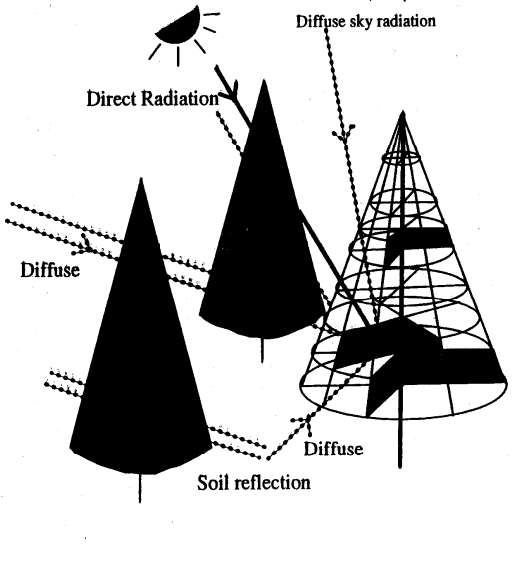
\includegraphics[width=0.5\textwidth]{/home/mn811042/Thesis/chapter4/figures/cone_MAESPA.png}}
        
\caption{Representation of available crown shapes in MAESPA (a - f), except for ``box'', and a conical canopy representation in MAESPA from \citet{Medlyn2004} (g).}
\label{f:crown_shapes}
\end{figure}


A number of grid points are located in a target crown and radiation at those grid points is calculated based on shading within the crown, shading by neighbouring trees, the solar zenith ($\theta$ = 45$^{\circ}$) and azimuth ($\varphi$ = 0$^{\circ}$) angle and whether radiation is direct or diffuse (Fig.~\ref{f:crown_shapes}g). Scattering of radiation is approximated following \citet{Norman1979}. 

Previous studies \citep{Oker-Blom1982,Kuuluvainen1987} showed that there were small differences (less than 5\%) in absorbed PAR by crowns of a reasonably wide range of ellipsoidal shapes. In the present sensitivity analysis, the differences in absorbed PAR between different crown shapes were limited to about 10\% between a box (fAPAR$_{box}$ = 0.26) and a conical (fAPAR$_{cone}$ = 0.15) shape. All the other crown shapes presented values of fraction of absorbed PAR of the order of 0.24. 

The conical crown shaped canopy also showed an approximately 17\% higher direct transmittance in comparison to the uniform box shape and a decrease in reflectance. This is a relevant result to be taken into account in boreal coniferous forests, for example. These forests usually present increased PAR soil albedo during winter in the presence of snow and a substantial mutual shadowing between the needles of a shoot. An increased direct transmittance associated with a conical crown shape in the presence of snow could result in even more backscattered radiation, and more PAR absorption. These regions of the world are light limited in great part of the year and this behaviour could help trees to absorb more radiation.  
  
The same idea of exploring different structural properties can be applied to leaf angle distributions. For this experiment, the leaf angle distribution (G-function) within crowns was written following six probability distribution functions ($g^{\prime}(\theta_l)$)  described by \citet{deWit1965}: (i) \textit{spherical} or random, where the relative frequency of leaf angle is the same as for surface elements of a sphere; (ii) \textit{planophile}, where horizontal leaves are most frequent; (iii) \textit{erectophile}, where vertical leaves are most frequent; (iv) \textit{plagiophile}, where oblique ($\theta_l$ $\approx$ 45$^{\circ}$) leaves are most frequent, (v) \textit{extremophile}, where oblique leaves are least frequent, i.e., mostly horizontal or vertical leaves; and (vi) \textit{uniform}, where the proportion of leaf angle is the same at any angle (Fig.~\ref{f:g_function}). 

\begin{figure}[ht]
      	\centering
        \includegraphics[width=1\textwidth]{/home/mn811042/src/pySellers/g_function_fontsize_24_2.png}
        \caption{Leaf angle distribution function is described as the proportion of leaves ($g^{\prime}(\theta_l)$ function) for different angles.} 
\label{f:g_function}
\end{figure}

In MAESPA the leaf angle distribution used in the radiative transfer calculations can be specified by:

(a) the number of leaf angle classes (N$\alpha$) and the ratio of the horizontal and vertical axes of an ellipsoid ($\chi$), which is the parameter of an ellipsoidal leaf angle distribution \citep{Campbell1990}. If N$\alpha$ = 1, there is only one leaf angle class with an average angle ($\overline{\theta_l}̅$). If N$\alpha$ $>$ 1, ($\overline{\theta_l}̅$) is used to generate the leaf inclination angle distribution assuming an elliptical distribution.

(b) If $\chi$ = 1, the distribution is \textit{spherical}; if $\chi$ = 0.5, the distribution is \textit{erectophile}; and if $\chi$ = 2, the distribution is \textit{planophile}. 

(c) Alternatively, the proportion of leaf area in each angle class can be read from an array (F$\alpha$). 

MAESPA can take up to nine possible leaf angle classes and the distribution of angles is elliptical following the parameter $\chi$. The default is N$\alpha$ = 1 and $\chi$ = 1, i.e. one leaf angle class following a \textit{spherical} distribution. 

For the particular evaluated canopy, the leaf angle distribution (G-function) caused a difference of up to 4\% in absorbed PAR, 17\% in direct transmitted PAR and less than 1\% in reflectance. The biggest difference caused by the G-function on radiation partitioning was between the \textit{erectophile} and \textit{planophile} distributions as expected once these two distributions are the opposite (vertical vs. horizontal leaves). 

A canopy with most leaves in the vertical position (\textit{erectophile}) allows more radiation goes through it with fewer interactions (fAPAR = 0.25) than a canopy with most leaves in the horizontal position (\textit{planophile}), which blocks more direct light and presents more absorption (fAPAR = 0.29). All the other distributions are somewhere in between these two. 

Finally, the geometrical impact on radiation partitioning due to the position of the Sun in the sky is well understood  and described by the radiative transfer theory, but still needs to be explored when analysing it over open forest canopies with heterogeneous structural features.

The position of the Sun in relation to the zenith (the point in the sky or celestial sphere directly above an observer) gives the so called solar zenith angle and describes the position in which the Sun is located in the celestial sphere. In order to have a precise position of the Sun, the observer needs a combination of two different types of information: firstly, the Solar Zenith Angle ($\theta$), and second the Solar Azimuth Angle ($\varphi$), defined as the position of the Sun in relation to the North, where 0$^{\circ}$ indicates the Sun is in the North. In this case, azimuthal variations were excluded of the analysis, because the optical depth of a vegetation canopy is mostly affected by zenithal variations. $\varphi$ was set 0$^{\circ}$. 

When the source of radiation is right above a heterogeneous vegetation canopy, the radiation has less material to interact in the presence of more gaps. As the solar zenith angle increases the path length of the radiation increases and because there is more material in this path length the optical depth of the canopy increases as well. This effect can be observed by the radiation partitioning evaluated in Fig.~\ref{f:balance_gort} with solar zenith angle varying. 

The direct transmittance decreases because the between-crown gaps are less observable in high solar zenith angles, and in this particular case the direct transmittance is mainly caused by within-crown gaps. As the direct transmittance decreases the absorption increases because there is more plant elements being illuminated. Finally, the reflectance also decreases because there is less direct radiation reaching the background soil and being upscatered isotropically, and more absorbing material on the radiation path way out of the vegetation canopy.

For this specific canopy in proportional terms, radiation absorption peaks when the solar zenith angle is around 85$^{\circ}$ in 60\%, as well as transmittance decreases to a minimum of around 40\%. The variation in both terms for all possible solar zenith angles (0$^{\circ}$ - 90$^{\circ}$) is of about 35\%. Reflectance goes from about 10\% in when the solar zenith angle is 0$^{\circ}$ to about half of that by 85$^{\circ}$. The extreme end of the solar zenith angles range, from approximately 85$^{\circ}$ to 90$^{\circ}$, has a different behaviour from the rest of the curve mainly because of edge effects. If the canopy was infinite, or the crown centres were immediately close to the ground this effect could be minimised. 

Indeed angular variations are one of the most important variables when studying radiative transfer in forest canopies, especially heterogeneous ones. The idea behind a factor that accounts for structural effects of vegetation on radiation partitioning is well accepted by the scientific community and often taken into account when calculating radiative transfer for different purposes. However, the angular variation of this ``correction factor'' is still an open debate and needs to be further explored. 

As discussed before, the presence of an angular dependence of clumping index could improve considerably the radiation partitioning of simpler 1D radiative transfer models because structural canopy features depend on observation or incident radiation angles. 

The following section explores the sensitivity analysis developed in here through an index proposed by \citet{Hoffman1983} in order to mathematically characterise the impact of each one of the evaluated variables on the radiation partitioning in 3D radiative transfer models. 

\subsection{`Local' sensitivity analysis of related canopy radiative transfer variables}\label{section:local}
Usually authors \citep{Downing1985,Iman1988} use the terms `sensitive', `important', `most influential', `major contributor', `effective', or `correlated' interchangeably to refer to the degree to which an input parameter affects the model output \citep{Hamby1994}.

\citet{Crick1987} have made a distinction by referring to `important' parameters as those whose uncertainty contributes substantially to the uncertainty in assessment results, and `sensitive' parameters as those which have a significant influence on assessment results. The consensus among authors is that models are indeed sensitive to input parameters in two distinct ways: (1) the variability, or uncertainty, associated with a sensitive input parameter is propagated through the model resulting in a large contribution to the overall output variability, and (2) model results can be highly correlated with an input parameter so that small changes in the input value result in significant changes in the output \citep{Hamby1994}.

Conceptually, the simplest method to perform a sensitivity analysis is to repeatedly vary one parameter at a time while holding the others fixed \citep{Downing1985,Crick1987}. A sensitivity ranking can be obtained quickly by increasing each parameter by a given percentage while leaving all others constant, and quantifying the change in model output. This type of analysis has been referred to as a `local' sensitivity analysis \citep{Crick1987} since it only addresses sensitivity relative to the point estimates chosen and not for the entire parameter distribution. 

A simple method of determining parameter sensitivity is to calculate the output percentage difference when varying one input parameter from its minimum value to its maximum value \citep{Hoffman1983,Bauer1991}. \citet{Hoffman1983} advocate the use of each parameter$^{\prime}$s entire range of possible values in order to assess true parameter sensitivities. The `sensitivity index' (SI) is calculated using,
\begin{equation}
SI = \frac{D_{max}-D_{min}}{D_{max}}
\label{equation:si}
\end{equation}
\noindent where $D_{min}$ and $D_{max}$ represent the minimum and maximum output values, respectively, resulting from varying the input over its entire range \citep{Hoffman1983}. This figure-of-merit provides a good indication of parameter and model variability.

\begin{figure}[ht!]
\centering
\begin{tabular}{ll}
\subfloat[Absorption]{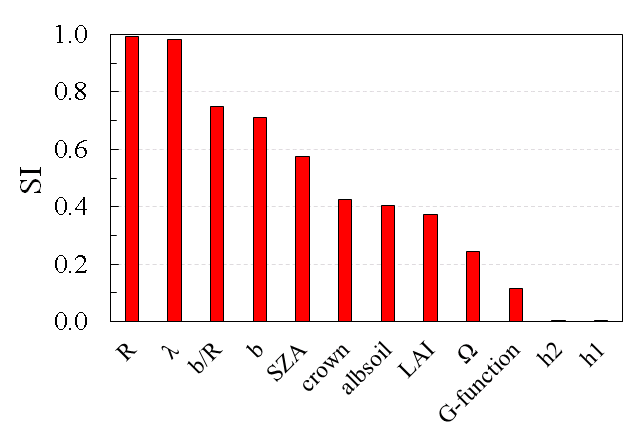
\includegraphics[width=0.5\textwidth]{/home/mn811042/Thesis/chapter4/figures/SI_absorbance.png}}
&
\subfloat[Reflectance]{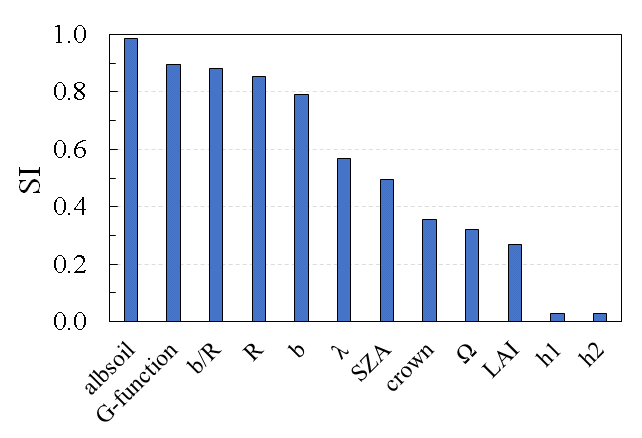
\includegraphics[width=0.5\textwidth]{/home/mn811042/Thesis/chapter4/figures/SI_reflectance.png}}
\end{tabular}
\subfloat[Transmittance]{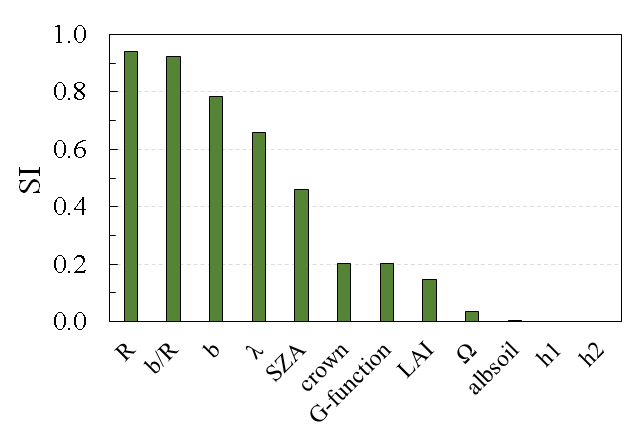
\includegraphics[width=0.5\textwidth]{/home/mn811042/Thesis/chapter4/figures/SI_transmittance.png}}
\caption{‘Local’ sensitivity analysis of 12 parameters described in Table~\ref{tab:parameters_gort} through the evaluation of the ‘Sensitivity Index’ (SI) \citep{Hoffman1983} for the terms of the radiation partitioning of PAR a) absorption, b) reflectance and c) transmittance.}
\label{f:si_radiationpartitioning}
\end{figure}

Fig.~\ref{f:si_radiationpartitioning} shows the sensitivity index for 12 parameters related to canopy structure, geometry, spectral and optical properties detailed described in Table~\ref{tab:parameters_gort}. As the analysis performed in the previous section, the sensitivity index rank the variables from 0, which indicates the model results are not well correlated with an input parameter and 1, which indicates high correlated parameters, so that small changes in the input value result in significant changes in the terms of the PAR radiative partitioning evaluated with the models GORT and MAESPA. Sensitivity in here follows the second meaning described by \citet{Hamby1994}, where changes in the input value (x-axis) result in significant changes in the output.

In terms of absorption, Fig.~\ref{f:si_radiationpartitioning}a indicates that the parameters $R$, horizontal crown radius, and $\lambda$, tree density, are responsible for the most significant changes, followed by two other structural parameters, $b/R$ and $b$. The `local' sensitivity analysis reinforce the fact that canopy structure is the most important factor influencing PAR absorption. Solar zenith angle (SZA) comes in the fourth place and indicates a strong influence of Sun geometry. 

The same type of behaviour is observed when analysing transmittance (Fig.~\ref{f:si_radiationpartitioning}c), where the most influential variables are the ones related to canopy structure, followed by the position of the radiation source. The difference however is related to the fact that crown ellipsoidal shape defined by horizontal crown radius ($R$), the vertical to horizontal crown radius ratio ($b/R$) and the vertical crown radius ($b$) are more influential over transmittance than tree density itself. 

In terms of canopy albedo, or reflectance (Fig.~\ref{f:si_radiationpartitioning}b), the soil albedo is the most influential parameter. It is important to highlight the vegetation canopy cover of 20\% when evaluating canopy albedo. That means 80\% of the scene (top view) is bare soil and because of that, the soil albedo is very impacting on canopy reflectance. This result would be probably different if the evaluated canopy was denser with higher canopy cover.

Perhaps one of the most important messages to take from the analysis performed here is the fact that solar zenith angle has always a greater impact than LAI for all the three terms of the radiation partitioning, absorption, reflectance and transmittance. 

The LAI is frequently used in 1D radiative canopy models as a parameter to determine the optical depth of a homogeneous canopies. But is the LAI a sufficient parameter to describe the optical depth of a real heterogeneous forest canopy? The next section explores the ability of LAI in taking into account structural heterogeneity on shortwave radiation partitioning. 

\subsection{Can LAI take into account vegetation canopy structural variability?}\label{section:lai}
Even though a large number of advances were used to improve canopy radiative transfer models, the most impacting variable to describe vegetation depth in radiative transfer schemes commonly used in current climate and weather forecast models is the leaf area index, or the LAI \citep{Yang2001}.

The typical values of LAI can vary from 1 to 9 m$^2$.m$^{-2}$ for a broadleaf forest, or from 1 to 3 for scrubs \citep{Clark2011}. In order to identify variations in fraction of absorbed PAR (fAPAR) related to different factors associated with canopy structure, a more specific analysis was conducted based on a previous experiment proposed by \citet{pinty2006} for three different vegetation conditions (Fig.~\ref{f:3d_maespa}), using a 1D radiative transfer model where the vegetation canopy is treated as turbid medium, the Two-Stream scheme \citep{Sellers1985}, and a 3D radiative tree based model, MAESPA \citep{Duursma2012}. In this experiment a fixed value of LAI of 3.2 m$^2$.m$^{-2}$ and a range of different parameters were set up and are described in Table~\ref{tab:parameters_laisense}.

\begin{threeparttable}
\centering
\caption{Variables defining the structurally heterogeneous scenes.}
%\begin{tabular*}{\textwidth}{ l@{\extracolsep{\fill}}*{4}{c}}
\begin{tabular}{l{0.25\textwidth} l{0.75\textwidth}}
%\begin{tabular}{\textwidth}{|p{\textwidth/4}|p{\textwidth/4}|p{\textwidth/4}|p{\textwidth/4}|}
%\begin{tabular*}
     \hline
     \hline
\textbf{Variable Identification}   & \textbf{Values (Units)}\\
\noalign{\smallskip}\hline
Mean Leaf Area Index over the domain         &	3.19$^S$, 3.19$^M$ and 3.15$^D$ (m$^2$.m$^{-2}$)\\
Mean Leaf Area Index of a single tree crown  &	6.02$^S$, 2.25$^M$ and 0.21$^D$ (m$^2$.m$^{-2}$)\\
Tree density 	                             & 53$^S$, 142$^M$ and 4718$^D$ (trees/ha)\\
Mean tree height	                     &23.99$^S$, 24.49$^M$ and 9.92$^D$ (m)\\
Mean tree crown height	                     &7.59$^S$, 7.09$^M$ and 7.57$^D$ (m)\\
Spatial distribution of tree locations	     & Random distribution\\
Crown shape	                             & Ellipsoid\\
Soil reflectance$^a$	                     & 0.100\\
Leaf reflectance$^a$	                     & 0.082\\
Leaf transmittance$^a$ 	                     & 0.093\\
\hline
\hline%\noalign{\bigskip}
%\end{tabular*}
\end{tabular}
\begin{tablenotes}
      \small
      \item $^S$Sparse vegetation. $^M$Medium vegetation. $^D$Dense vegetation. 
      \item $^a$ PAR wavelength (400 - 700 nm). 
\end{tablenotes}
\label{tab:parameters_laisense}
\end{threeparttable}

\bigskip
%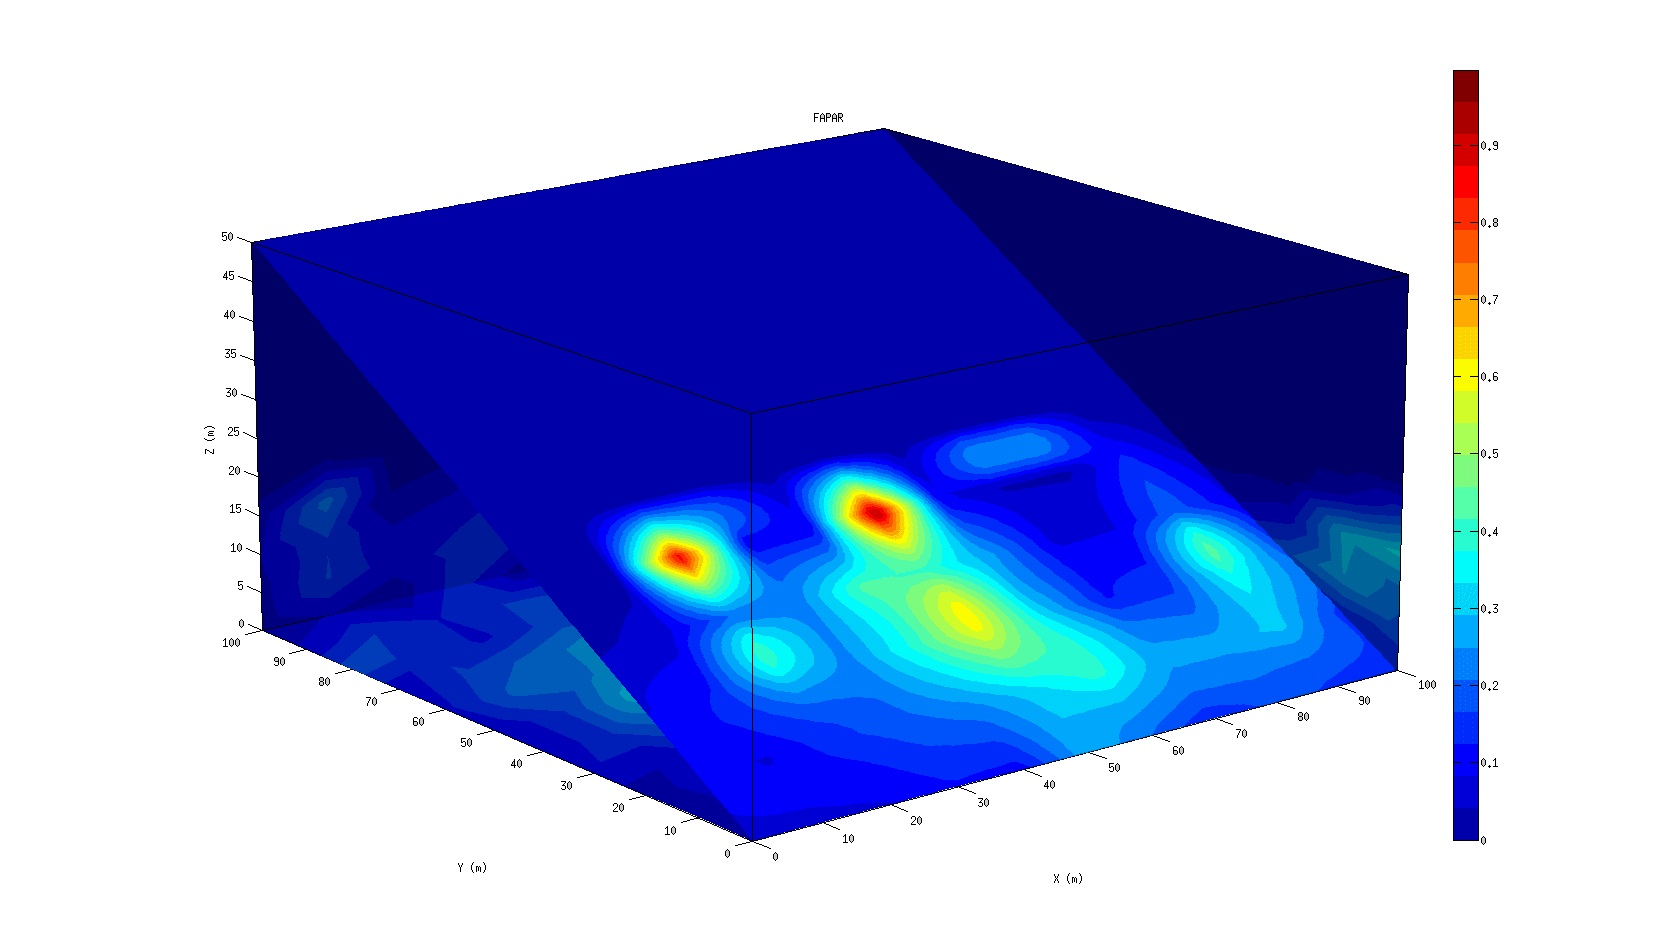
\includegraphics[width=0.6\textwidth]{/home/mn811042/Thesis/chapter4/figures/FAPAR_sparse.png}
\begin{figure}
\centering
\begin{tabular}{ll}
\subfloat[Sparse Canopy]{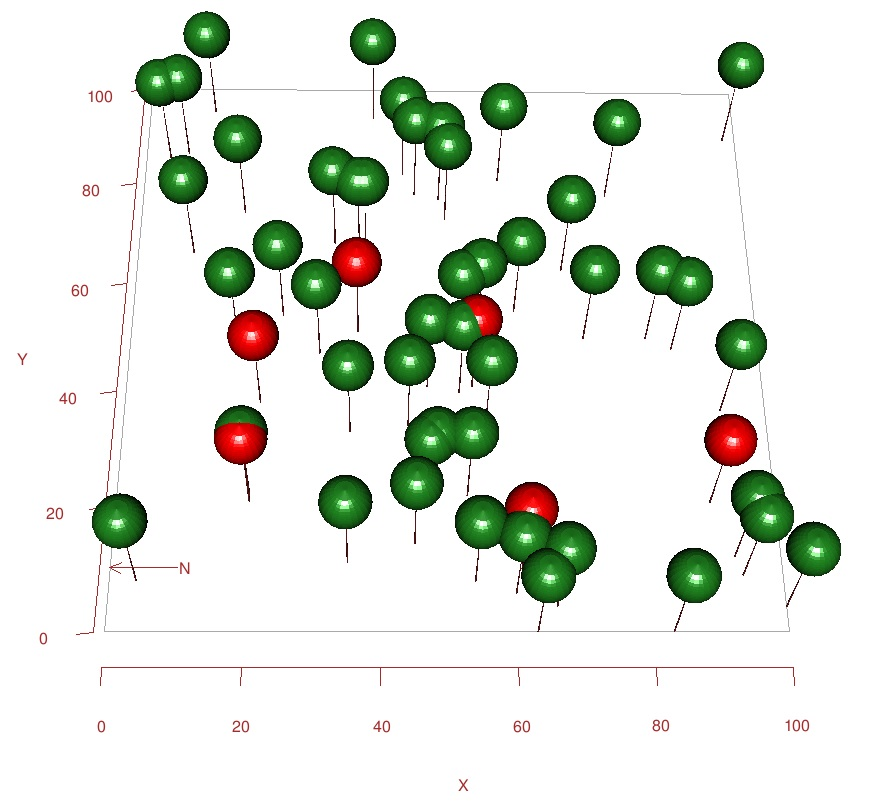
\includegraphics[width=0.40\textwidth]{/home/mn811042/Thesis/chapter4/figures/sparse_1.png}
                         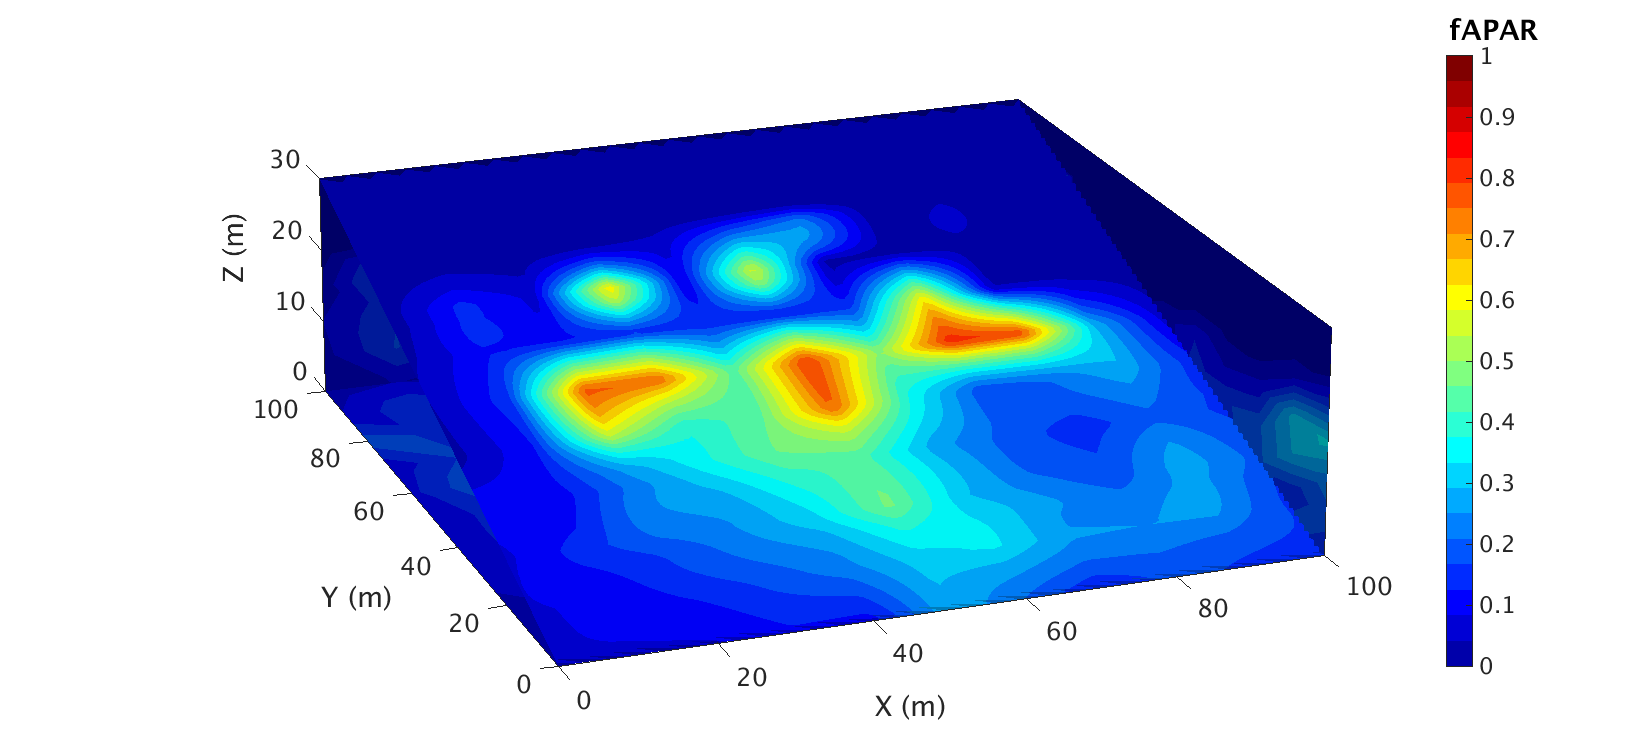
\includegraphics[trim=5cm 0cm 0cm 0cm,angle=0,clip=True,width=0.60\textwidth]{/home/mn811042/Thesis/chapter4/figures/3D_fapar_sparse.png}}
\end{tabular}

\begin{tabular}{ll}
\subfloat[Medium Canopy]{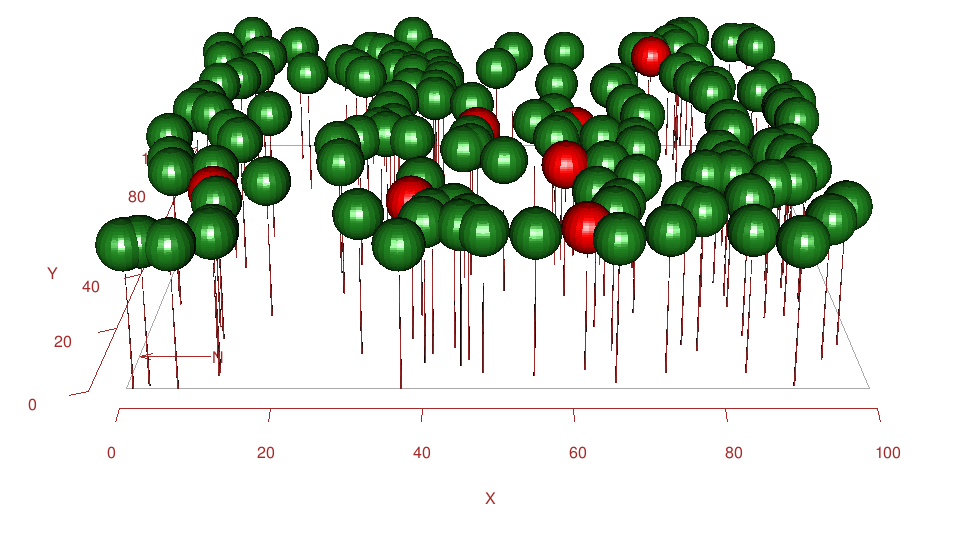
\includegraphics[width=0.45\textwidth]{/home/mn811042/Thesis/chapter4/figures/medium_1.png}
                         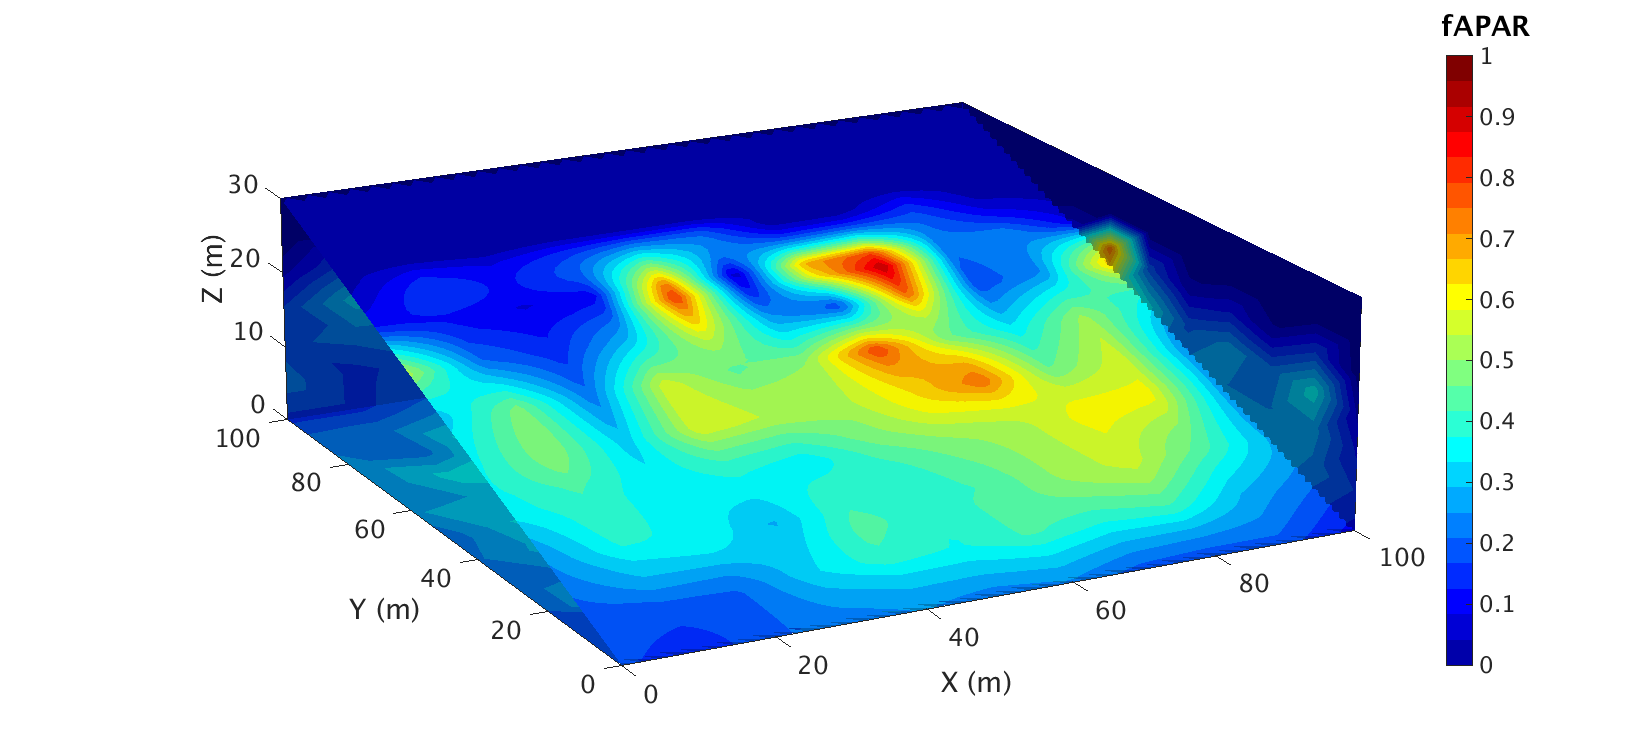
\includegraphics[trim=5cm 0cm 0cm 0cm,angle=0,clip=True,width=0.55\textwidth]{/home/mn811042/Thesis/chapter4/figures/3D_fapar_medium.png}}
\end{tabular}

\begin{tabular}{ll}
\subfloat[Dense Canopy]{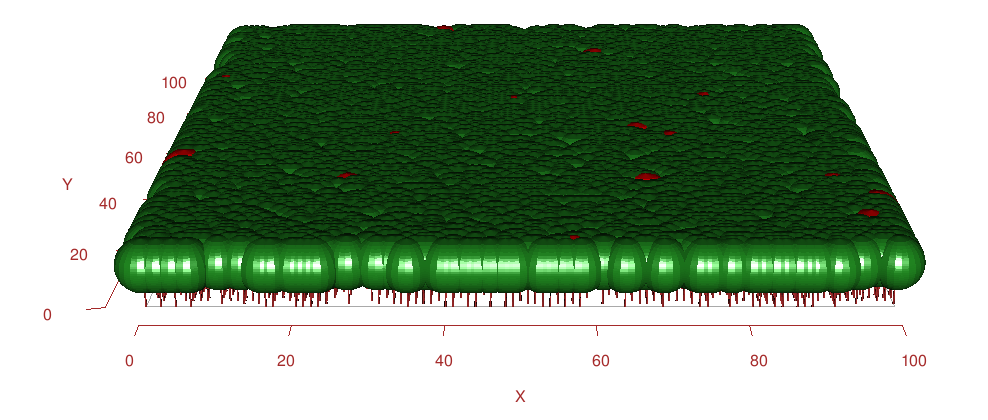
\includegraphics[width=0.45\textwidth]{/home/mn811042/Thesis/chapter4/figures/dense_1.png}
                        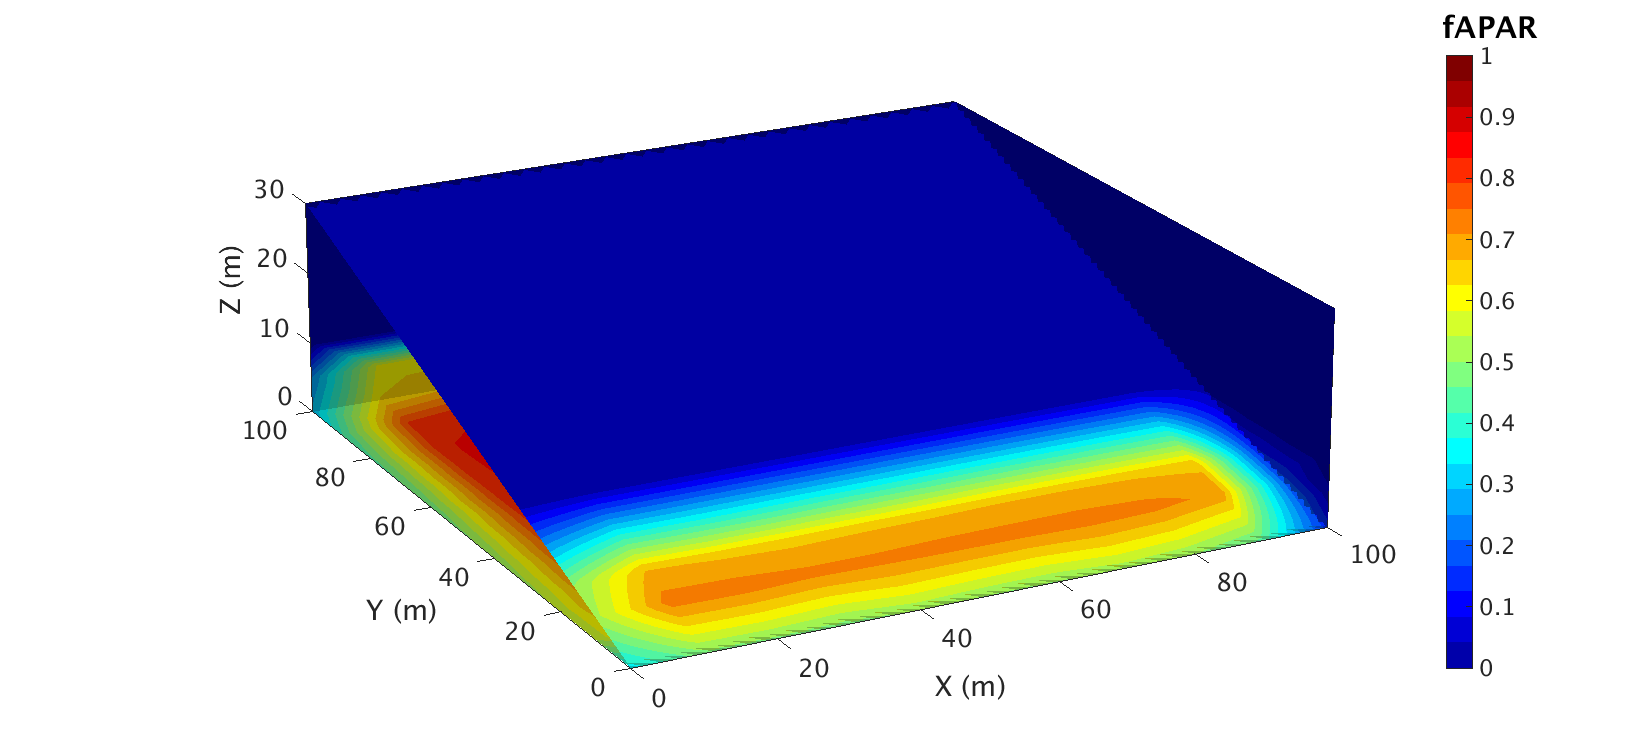
\includegraphics[trim=5cm 0cm 0cm 0cm,angle=0,clip=True,width=0.55\textwidth]{/home/mn811042/Thesis/chapter4/figures/3D_fapar_dense.png}}
\end{tabular}
\caption{a. One hectare (100 m x 100 m) of three different canopy densities: sparse, medium and dense. Red trees represent target trees, i.e., trees reached by radiation (left); b. 3D profile of PAR absorption (right).}
\label{f:3d_maespa}
\end{figure}

Fig.~\ref{f:3d_maespa} shows a 3D representation of each one of the three canopy densities, where red trees indicate the target trees. The selection of randomly distributed target trees within a vegetation canopy is a method implemented to save computational time when running the 3D tree based model MAESPA, but without compromising the final results. 

As MAESPA calculates the radiative balance, water balance and surface energy balance for each single tree present in the canopy, the amount of computational time spend in a very dense canopy can be relatively long. Using fewer target trees for complete flux calculations and surrounding trees when calculating the mutual crown shading of the target tree does not alter the final results in radiation absorption, as evaluated in edge experiments. 

The 3D profile of PAR absorption can be spatially different for each one the three canopy densities, even though the LAI is approximately constant between them ($\approx$ 3.2 m$^2$.m$^{-2}$). For the sparse case, few tree crowns are responsible for large amounts of absorbed radiation with several spots with no absorption at all, especially at the bottom of the canopy. For the dense case, radiation absorption behaves almost uniformly within the 3D space, with large values at the centre and top of the canopy. The border effect plays a role here once the canopies are finite and radiation is direct. The borders show less absorption because of less mutual shading. 

The same LAI value was used in the Two-Stream scheme (\textbf{TS}) under two different sky conditions: totally diffuse light (\textbf{TS isotropic}) and direct light (\textbf{TS direct}). Under an isotropic illumination condition, the Two-Stream output value of fraction of absorbed photosynthetically radiation (fAPAR) is constant (fAPAR $\approx$ 0.9) with solar zenith angle. For direct illumination, the fAPAR varies from 0.77 to 0.93 and it is systematically lower than the diffuse condition until a solar zenith angle of approximately 60$^{\circ}$ (Fig.~\ref{f:ts_maespa}).

In comparison to MAESPA (isotropic illumination condition), both Two-Stream scenes are overestimating the fAPAR values, which indicates that 3D representations are more `transparent' than their 1D equivalent with respect to the direct transmitted radiation. Although, for a dense canopy under illumination angles between 0$^{\circ}$ and 40$^{\circ}$, fAPAR values obtained by MAESPA and TS direct are comparable. That indicates a relatively accurate performance of the Two-Stream scheme in partitioning PAR in densely vegetated canopies, such as tropical rainforests, for example. However, in sparser canopies with same LAI, the TS method seems to overestimate fAPAR in 25\% for medium vegetated canopies and up to 50\% for sparse vegetated canopies. 

The results showed in this section highlight the limitations of the Two-Stream radiative transfer scheme in reproduce the results of a 3D tree based model for PAR absorption based on LAI only. This section points out to the need for a different approach to consider canopy structural variability that is not captured just by the use of LAI. 

\begin{figure}
\centering

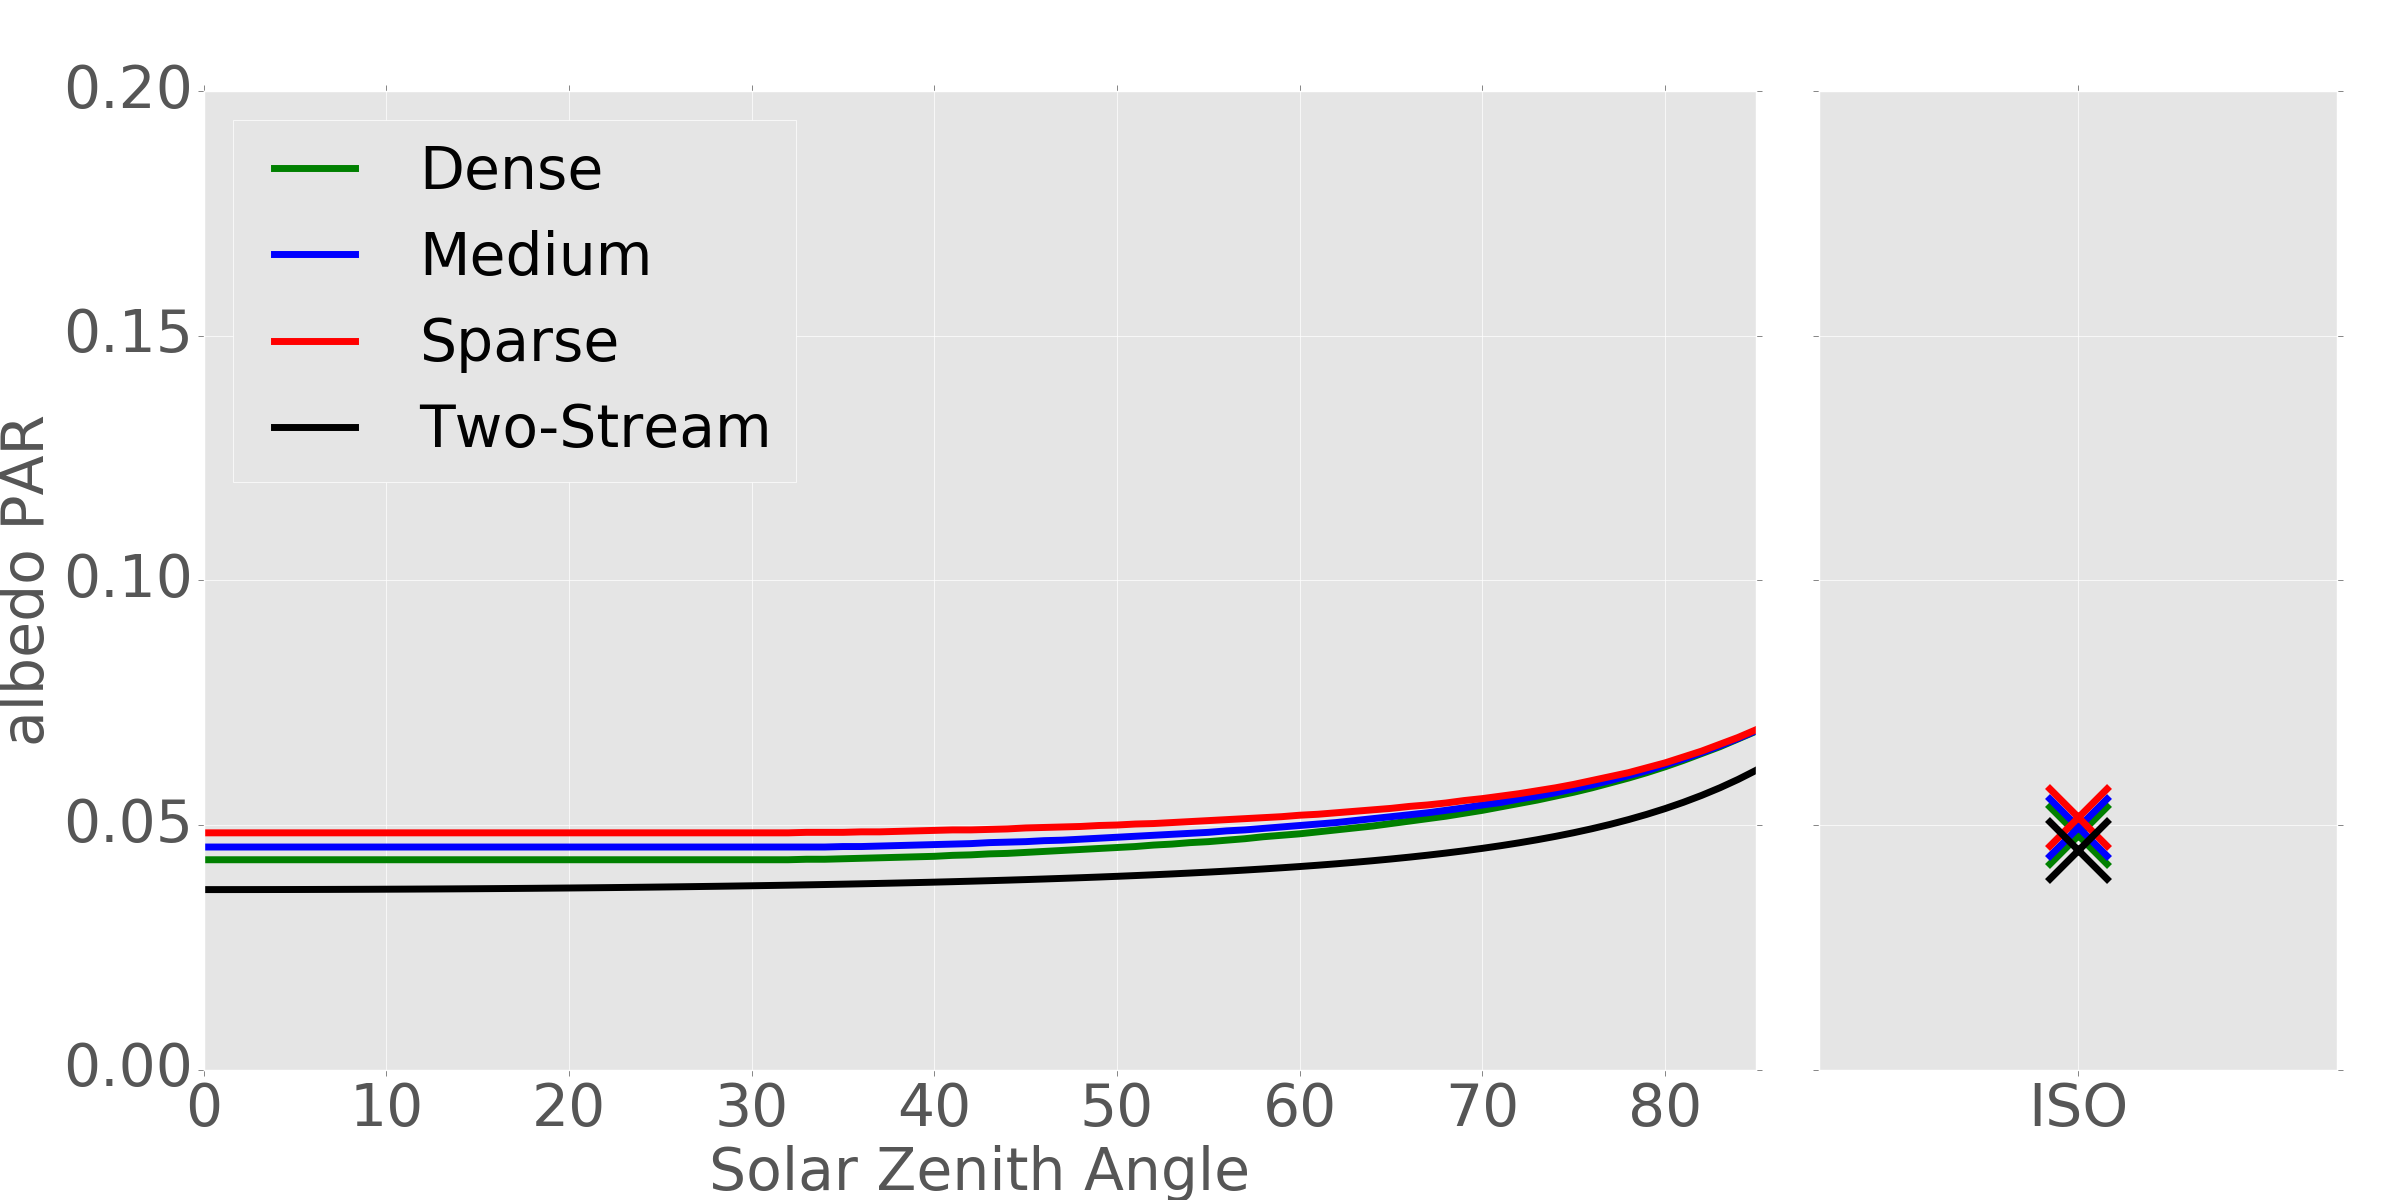
\includegraphics[width=0.5\textwidth]{/home/mn811042/Thesis/chapter4/figures/albpar_sza_lai_150_2.png}
\caption{Fraction of absorbed photosynthetically active radiation (fAPAR) with respect to the Two-Stream scheme (black lines) for a diffuse isotropic case (dashed line) and for a direct illuminated case (dash-dotted line). The colour lines represents three different vegetation canopies in MAESPA, described in Table~\ref{tab:parameters_laisense}.} 
\label{f:ts_maespa}
\end{figure}

\section{Considering structural effects in 1D radiative transfer treatments: parameterisations}\label{section:parameterisations}
Several previous studies have suggested with observations and detailed modelling approaches that vegetation three-dimensional (3D) structure influences radiation partitioning and other land surface related processes \citep{Nilson1971,Wang1990,Chen1996,Kucharik1999,Yang2001,Yang2003,Jonckheere2004,pinty2006,Chen2008,Ni-Meister2010,Widlowski2011,Kobayashi2012,Loew2014}.

For most natural woody vegetation such as conifers and savannahs, the spatial distribution of individual tree crowns creates clear spaces where beam radiation propagates without interference of vegetation elements, and because of that the Two-Stream scheme (vertical 1D) results in large deviations from the actual amounts of absorbed and reflected radiation \citep{Ni-Meister2010,Kobayashi2012,Loew2014}.

For detailed computation of 3D radiation fields within complex vegetation canopies, radiative transfer schemes can use a geometrical optical approach and treat mixtures of individual trees and multiple scattering with foliage clumped within tree crowns, e.g. in the GORT model \citep{Li1995}, or heterogeneously between tree crowns, e.g. in MAESTRA/MAESPA \citep{Wang1990,Duursma2012}, among others more complex approaches. However, these models cannot be directly used in GCMs due to their extreme computational power demand \citep{Yang2001} and the high number of required vegetation structural parameters \citep{Loew2014}. 

Even though efficient 1D radiative transfer schemes are still preferably used, because of their simplicity, speed and suitability to run over large areas, the use of effective radiative state variables to express the properties of 3D vegetation canopy systems makes a simpler model to analogously simulate the radiation balance of more complex 3D models \citep{Pinty2004,pinty2006}. 

This requirement is not specific to vegetation canopy systems, but can be applied to all structurally heterogeneous radiative medium, like clouds, for example.

The probability of the transmission of a beam light through a vegetation canopy has been commonly described by the gap fraction theory firstly proposed by \citet{Monsi1953,Monsi2005}: 
\begin{equation}
P_{gap}(\theta) = \exp{\Big(\frac{-G(\theta) \cdot LAI \cdot \Omega}{\cos{\theta}}\Big) = \exp{\Big(\frac{-G(\theta) \cdot L_e}{\mu}\Big)}
\label{equation:pgap}
\end{equation}
\noindent where P$_{gap}(\theta)$ is the direct transmittance, $\theta$ is the solar zenith angle, $\mu$ is the cosine of $\theta$, G($\theta$) is the `G-function' defined as the leaf projection function on the plane perpendicular to the view direction \citep{WarrenWilson1960,Ross1981,Sellers1985,Myneni1989} and often assumed to be a spherical distribution of leaf normals \citep{Chen1992,Chen2012}. $L$ is the `true LAI' and $\Omega$ is the `clumping index' firstly proposed by \citet{Nilson1971}, but revisited by many other authors to account for structural heterogeneity associated with the evaluated vegetation canopy. Therefore, $L_e$ is referred as the `effective LAI', a domain-averaged quantity, that can be forced to satisfy the main constraints associated with a 1D representation by any factor accounting for structural variability in a determined turbid medium.

Thus $L_e$ accounts for all phyto and woody elements composing the vegetation canopy, and when its value exceeds the true LAI, it is an indication of specific structural canopy conditions associated with significant amounts of woody elements \citep{pinty2006}. 

The `clumping index' \citep{Nilson1971,Norman1974,chen1992,Chen1996} is associated with the heterogeneous nature of the canopy volume, often used at the tree resolution, and revisited later on by other authors \citep{Pinty2004,pinty2006}, who used the same scientific proposition to account for structural heterogeneity of different radiative media at stand scale, specially in association with satellite products.

Few other authors \citep{Kucharik1999,pinty2006,Ni-Meister2010} attempted to formulate simplified modelling approaches to resolve vegetation clumping at several levels of organisation, in order to address one major difficulty associated with radiative transfer in non-homogeneous forest canopies all over the world.

The next sections will describe and evaluate 3 different propositions top address vegetation clumping in 1D radiative transfer schemes. Evaluations will be performed against a benchmarking exercise of radiation transfer in vegetation canopies, the RAMI4PILPS experiment \citep{Widlowski2011}.

\subsection{The clumping index by Kucharik et al. (1999)}
The parameterisation described in this subsection was developed by \citet{Kucharik1999}. The authors used measurements of LAI and gap fraction made with MVI (Multiband Vegetation Imager) \citep{Kucharik1997} obtained during the BOREAS (Boreal Ecosystem-Atmosphere Study) \citep{Sellers1997} field campaigns of 1994-1996 to derive a semi-empirical relationship between $\Omega(\theta)$ and solar zenith angle ($\theta$). 

In this method, two key quantities are needed: (i) the fraction of ground area covered by the horizontal projection of crown envelopes ($f_c$) (from nadir view), which is a function of the typical tree crown diameter ($D$), and tree stem spacing ($\lambda$), or stem density, within a study plot; and (ii) an estimate of crown porosity ($\Phi$); this quantity is related to foliage density and defined as the gap fraction within crown envelopes divided by $f_c$.
 
A series of zenith gap fraction measurements were needed along a transect beneath a canopy to partition the total gap fraction ($f_{gap},t(0)$) between within-crown and between-crown gaps, and  an estimate of the total fraction of ground area covered by the horizontal projection of crown envelopes ($f_c$). To obtain $f_c$, the typical crown silhouette area ($\pi R^2$, where $R$ is the crown radius in the horizontal direction) is multiplied by the number of crowns and divided by the total ground unit area on which the stem density is based. If $f_c$ is greater than 1, crowns typically overlap in the forest, and the entire value of $f_{gap},t(0)$ can be defined as within-crown gap fraction ($f_{gap},c(0)$). The total gap fraction occurring between-crowns ($f_{gap},b(0)$) can be estimated by $1 - f_c$, and $f_{gap},c(0)$ is therefore approximated by $f_{gap},t(0) - f_{gap},b(0)$. If the value of $f_{gap},c(0) < 0$, it can be assigned a value of 0 for all practical purposes. 

Crown porosity ($\Phi$) is determined by dividing $f_{gap},c(0)$ by $f_c$ ($\Phi$ = $f_{gap},c(0)/f_c$). The value of $\Phi$ may be described as a normalised within-crown gap fraction. Generally, an error of about 0.05 exists in determining $f_c$ and $\Phi$ by using an average crown radius and tree stem density rather than the actual model calculations of $f_c$. However, the authors indicated that these errors are not of concern when estimating $\Omega(0)$ using the gap-fraction partitioning strategy.

Values of $\Phi$ and $f_c$ were then used to determine a value of $\Omega$(0) that was consistent with calculations resulting from numerical simulations of the canopy gap-size distribution. A non-linear least-squares fit to approximately 250 Monte Carlo simulations (analysing values of $\Omega(0)$) was performed for values of $f_c$ $\geq$ 0.20, and for all simulated values of $\Phi$. A separate fit to the entire set of model data was performed for 0.04 $\geq f_c \geq$ 0.30. For sparse canopies where $f_c < 0.20$, a value of $\Omega(0)$ could still be determined. 

Ten equations were solved simultaneously to determine 10 coefficients ($a_0$, ..., $a_9$) that describe the relationship between values of $\Omega(0)$, $f_c$, and $\Phi$. To characterise the angular dependence of $\Omega(\theta)$, a minimum value of $\Omega(\theta)$ was determined at $\theta$ = 0$^{\circ}$ and a value of $\Omega(\theta)$ was needed at $\theta$ = 90$^{\circ}$. Because it was assumed that $\Omega(\theta)$ reaches its maximum value at $\theta$ = 90$^{\circ}$, \citet{Kucharik1999} refer to this value as the maximum possible element clumping index, $\Omega_{max}$, and defines it as:
\begin{equation}
\Omega_{max} = \Big(\frac{ND}{\sqrt{A}}\Big)^{0.7}
\label{equation:clumpmax}
\end{equation}
\noindent where $N$ is number of stems within ground area $A$, and $D$ is crown diameter. If $ND/\sqrt{A} > 1$, then the value of $\Omega_{max} = 1$. The angular dependence of $\Omega(\theta)$ was defined by \citet{Kucharik1999} following the equation: 
\begin{equation}
\Omega = \Omega(\theta) = \frac{\Omega_{max}}{[1 + b\exp(-k(\theta)^p)]}
\label{equation:clumptheta}
\end{equation}
\noindent where $k$ is constant (usually $k$ = 2.2), $\theta$ is zenith angle expressed in radians, and $b$ is solved from a rearrangement of Eq.~\ref{equation:clumptheta} using a known value of $\Omega(\theta)$ (e.g., $\theta$ = 0$^{\circ}$). A quantitative comparison of results produced using Eq.~\ref{equation:clumptheta} with the best-fit curves suggested that a value for $p$ can be approximated by an equation on the form:
\begin{equation}
p = -0.461\chi + 3.8
\label{equation:pchi}
\end{equation}
\noindent where $\chi$ is the ratio of crown depth to crown diameter. Generally, if $\chi$ is $\leq$ 1.0, $p$ = 3.34. 

This set of semi-empirical equations was used to estimate clumping index for three different canopy sets as in RAMI4PILPS (Table~\ref{tab:RAMI4PILPS}). The results calculated by Eq.~\ref{equation:clumptheta} are presented by dotted lines in Fig.~\ref{f:ci_comparisons}.

The range of clumping index obtained by this work was from approximately 0.2, for minimum Sun zenith angle (i.e. $\theta = 0^{\circ}$), with convergence to 1, for maximum Sun zenith angle (i.e. $\theta = 90^{\circ}$), for sparse and dense canopies, while the convergence in high solar zenith angles ($\theta > 70^{\circ}$ for the medium canopy was approximately 0.7, starting with very small $\Omega(\theta) \approx$ 0.0.

\subsection{The clumping index by Ni-Meister et al. (2010)}
Following the same attempt to derive a relationship for clumping index, \citet{Ni-Meister2010} developed an analytical prognostic expression based on stem density ($\lambda$), crown radius ($R$) and LAI. In here, only the equation used for sphere crowns is shown, however, the same authors extend the analysis to more generalised ellipsoid crowns, as introduced in \citet{Li1988}. The analytical solution for the modified clumping index in Beer$^{\prime}$s law is expressed as, 
\begin{equation}
\Omega = \gamma = \frac{3}{4\tau_0R}\Big(1 - \frac{1 - (2\tau_0R + 1)\exp(-2\tau_0R)}{2\tau_0^2R^2}\Big)
\label{equation:clumpNi}
\end{equation}
\noindent where $\tau_0r = 3 G LAI/ 4 \lambda \pi \cdot R^2$ for spherical crowns. 

The authors validated the analytical solutions for clumping factor with the ones calculated by the full GORT model \citep{Li1995}, which was specifically developed to describe the effects of 3D canopy structure on the radiative balance and to characterise the heterogeneous radiative balance in natural vegetation at the forest stand scale. 

This set of equations was used to estimate clumping index for three different canopy sets as in RAMI4PILPS (Table~\ref{tab:RAMI4PILPS}), as well. The results calculated by Eq.~\ref{equation:clumpNi} are presented by dashed-dotted lines in Fig.~\ref{f:ci_comparisons}. 

The canopy sets are defined in such a particular way (LAI increasing with density), that the resulting clumping index stayed constant for all cases. That indicates the `clumping index' from \citet{Ni-Meister2010} is not capable to identify structural differences associates with canopy density as proposed in the RAMI4PILPS exercise and it does not take into account different solar geometries.

\subsection{The structure factor parameterisation}
Among other parameterisations, the one proposed by \citet{pinty2006} presents a relatively ``self-sufficiency'', because it does not require any previous knowledge about vegetation structure, and because of that, it can be applied to any vegetation canopy. 

The values of the effective variables can be estimated by inverting a 1D radiative transfer model against the results obtained by a 3D model \citep{pinty2006}.

Previous studies have reported the dependency of `clumping index' on solar zenith angle \citep{Andrieu1993,Chen1996,Kucharik1999,Leblanc2005,Ryu2010}. This dependency remains rather smooth and limited \citep{Chen1997a,Chen1997} and it was written by \citet{pinty2006} following an approximated linear relationship:
\begin{equation}
\Omega = \zeta(\mu) \approx a + b \cdot (1 - \mu)
\label{equation:structurefactor}
\end{equation}
\noindent where $\mu$ is the cosine of $\theta$, $a = \zeta(\mu=1)$ is the parameter corresponding to an overhead Sun, and $b$ the parameter responsible for include the effects of a range of different Sun geometries.

In the particular case of an overhead Sun ($\theta$ = 0$^{\circ}$), $a$ is also equal to:
 \begin{equation}
\zeta(\mu=1) = -\ln{(1 - F_c)}\frac{2}{LAI}
\label{equation:structurefactora}
\end{equation}
\noindent where $F_c$ is the true vegetation cover (accounting for within and between crown gaps) obtained for a Black Canopy representation ($\rho_{leaf} = \tau_{leaf} = 0.0$) of the total incident radiation minus direct transmissivity with an overhead Sun (1 - P$_{gap}(\theta = 0^{\circ}$)).
Both parameters are used to account for vegetation canopy heterogeneity and modify the radiation path length. 

The structure factor is introduced into the Two-Stream scheme by modifying three main groups of variables to account for canopy structural effects:

\begin{enumerate}
\item the optical depth of direct beam per unit leaf area, $K$; 
\item the average inverse diffuse optical depth per unit leaf area, $\mu$̅; and, 
\item the single scattering albedo, $a_s(\mu)$, used to obtain the upscattering parameters for the diffuse and direct beams, $\beta$ and $\beta_0$.
\end{enumerate}

The structure factor can be included on the optical depth of direct beam per unit leaf area, by modifying $K$ as:
\begin{equation}
K_{Structure}(\theta) = \frac{G(\theta)}{\mu} \cdot  \zeta(\mu)
\label{equation:opticaldepthstruct}
\end{equation}

The same analogy can be applied when calculating the average inverse diffuse optical depth per unit leaf area, $\bar{\mu}$, but obtaining the structure factor for the direction of scattered flux, $\mu^\prime$:
\begin{equation}
\overline{\mu_{Structure}} = \int_{0}^{1} \frac{\mu^\prime}{G(\mu^\prime) \cdot \zeta(\mu^\prime)} d\mu^\prime
\label{equation:muprimestruct}
\end{equation}

The parameter $\omega\beta$ can be inferred from the analysis of \citet{Norman1975} in the case of a single leaf whose normal is oriented at zenith angle $\theta_l$ from the local vertical defined in the upward hemisphere:
\begin{equation}
\omega\beta = \frac{1}{2}(\omega_l + \delta_l \cos^2 \theta_l)
\label{equation:omegabeta}
\end{equation}
\noindent where $\omega_l = \rho_{leaf} + \tau_{leaf}$ and $\delta_l = \rho_{leaf} - \tau_{leaf}$. 

The equation~\ref{equation:omegabeta} however is only valid for a single leaf and to obtain the total contribution of leaves over the canopy it is necessary to integrate over the appropriate leaf orientation probability distribution, between 0 and $\pi/2$, because the leaf normal are assumed to be oriented into the upward hemisphere, as in:
\begin{equation}
\omega\beta = \frac{1}{2}\Big(\omega_l + \delta_l \int_{0}^{\pi/2} \cos^2 \theta_l g^\prime(\theta_l) \sin \theta_l d\theta_l\Big)
\label{equation:omegabeta2}
\end{equation}
\noindent where $\sin\theta_l$ is introduced for normalisation requirement of the probability distribution function. And when isolating $\beta$, it is possible to obtain the generic diffuse upscatter parameter:
\begin{equation}
\beta = \frac{1}{2\omega}\Big(\omega_l + \delta_l \int_{0}^{\pi/2} \cos^2 \theta_l g^\prime(\theta_l) \sin \theta_l d\theta_l\Big)
\label{equation:beta}
\end{equation}

If the Two-Stream scheme equations are solved when $\lim_{\omega \to 0}$, i.e., single scatter approximation and semi-infinite canopy, the upward diffuse flux at the top of the canopy may be taken as equal to the single scattering albedo ($a_s(\mu)$). The equation for the direct upscatter parameter, $\beta_0$, is
\begin{equation}
\beta_0 = \frac{1 + \overline{\mu}K}{\omega\overline{\mu}K}a_s(\mu)
\label{equation:betazero}
\end{equation}

And $a_s(\mu)$ is given by, 
\begin{equation}
a_s(\mu) = \frac{\omega}{2}\int_{0}^{1} \frac{\mu^\prime G(\mu)}{\mu G(\mu^\prime) + \mu^\prime G(\mu)} d\mu^\prime
\label{equation:alphas}
\end{equation}

The equation above is just valid when assuming isotropic scattering for the leaf elements, which makes the scattering phase function independent of the angle of the incident beam (see \citet{Dickinson1983} and \citet{Sellers1985} for more details). 

The addition of the structure factor into the single scattering albedo formulation would result in,
\begin{equation}
a_s(\mu) = \frac{\omega}{2}\int_{0}^{1} \frac{\mu^\prime G(\mu) \zeta(\mu)}{\mu G(\mu^\prime) \zeta(\mu^\prime) + \mu^\prime G(\mu)\zeta(\mu)} d\mu^\prime
\label{equation:alphasstruct}
\end{equation}

In this case the formulation for the direct upscatter parameter considering canopy structure would be: 
\begin{equation}
\beta_0 = \frac{1 + \overline{\mu_{Structure}}K_{Structure}}{\omega\overline{\mu_{Structure}}K_{Structure}}
\bigg[\frac{\omega}{2}\int_{0}^{1} \frac{\mu^\prime G(\mu) \zeta(\mu)}{\mu G(\mu^\prime) \zeta(\mu^\prime) + \mu^\prime G(\mu)\zeta(\mu)} d\mu^\prime \bigg]
\label{equation:alphasstruct}
\end{equation}

\subsection{Minimising the `structure factor'}\label{sub:minimise}
The structure factor parameters were obtained for each canopy structure through the inversion of the Two-stream scheme against direct and diffuse fAPAR and albedo PAR reference values from the RAMI4PILPS experiment. The Nelder-Mead minimisation method \citep{Nelder1964}, or `downhill simplex' was used in the inversion process. 

To minimise the structure factor parameters in respect to canopy density, a minimum error evaluation was conducted varying $a$ and $b$ from 0.0 to 1.0 following the equation:
\begin{equation}
RMSE_{ab} = \sqrt{\frac{\sum_{n=1}^{N} (f_{Two-stream} - f_{MAESPA})^2}{N}}
\label{equation:rmseab}
\end{equation}
\noindent N = 85$^{\circ}$, $a$ = [0,1], $b$ = [0,1] and $f_{Two-stream}$ is the fAPAR calculated with the Two-stream radiative transfer scheme with the structure factor parameterisation for a combination of $a^{\prime}s$ and $b^{\prime}s$ and  $f_{MAESPA}$ is the fAPAR reference value calculated with the MAESPA model for different Sun zenith geometries varying from 0$^{\circ}$ to 85$^{\circ}$. fAPAR values from MAESPA have been validated (Fig.~\ref{f:szacomparisonfPAR}) and it seems to be a robust tool to calculate PAR absorption for different vegetation canopies, as it strongly agreed with the RAMI4PILPS reference values. 

The results showed in Figure~\ref{f:rmsd_ts_maespa} are limited to the PAR spectrum with a medium value of background albedo ($\alpha_{soil} = 0.12$). For all evaluated cases the combination of $a$ and $b$ that gives the minimum error between the 1D and the 3D cases is not a single value, but a combination of values described by a certain area of minimum Root-Mean-Squared-Error (RMSE). This finding suggests that for a determined forest stand there are a number of combinations of $a^{\prime}$s and $b^{\prime}$s that modifies the radiative transfer calculations of a 1D model and makes it matches the radiation partitioning of more complex 3D models. 

The sparse case seem to be equally sensitive to the parameters $a$ and $b$. As the canopy density increases, the sensitivity of $a$ starts to increase in relation to $b$, as it can be noticed by the larger error variation on the x-axis of $a$. This indicates that for denser canopies $b$ has reduced impact on architectural effects on radiation partitioning, if compared to $a$.

\begin{figure}
\centering
\begin{tabular}{lll}
\subfloat[LAI = 0.5 m$^2$.m$^{-2}$]{\includegraphics[width=0.33\textwidth]{/home/mn811042/src/julesRT_struct_2/julesRT_struct/RMSE_JULESRT_v2_MAESPA_050.png}}
\subfloat[LAI = 1.5 m$^2$.m$^{-2}$]{\includegraphics[width=0.33\textwidth]{/home/mn811042/src/julesRT_struct_2/julesRT_struct/RMSE_JULESRT_v2_MAESPA_150.png}}
\subfloat[LAI = 2.5 m$^2$.m$^{-2}$]{\includegraphics[width=0.33\textwidth]{/home/mn811042/src/julesRT_struct_2/julesRT_struct/RMSE_JULESRT_v2_MAESPA_250.png}}
\end{tabular}
\caption{Root-Mean-Squared-Error for Two-Stream scheme with the structure factor parameterisation and MAESPA for three canopies densities (sparse, medium and dense).}
\label{f:rmsd_ts_maespa}
\end{figure}

The structure factor parameters were obtained for each canopy density through inversion of fAPAR and albedo PAR values together over three soil backgrounds all together and are summarised bellow:

\begin{threeparttable}
\centering
\caption{Summary of the structure factor parameters minimised against the absorption and reflectance reference values for PAR waveband.}
\begin{tabular*}{\textwidth}{ l@{\extracolsep{\fill}}*{4}{c}}
%\begin{tabular}{{0.33\textwidth} {0.33\textwidth} {0.33\textwidth}}
%\begin{tabular}{\textwidth}{|p{\textwidth/4}|p{\textwidth/4}|p{\textwidth/4}|p{\textwidth/4}|}
%\begin{tabular*}
     \hline
     \hline
\textbf{Variable}   & \textbf{$a$} & \textbf{$b$}\\
\noalign{\smallskip}\hline
$\zeta_{sparse}(\mu)$ & 0.344 & 0.096\\
$\zeta_{medium}(\mu)$ & 0.337 & 0.256\\
$\zeta_{dense}(\mu)$  & 0.418 & 0.206\\
\hline
\hline%\noalign{\bigskip}
%\end{tabular*}
\end{tabular*}
\label{tab:structureparameters}
\end{threeparttable}
\bigskip

\section{Evaluating structural parameterisations}
Evaluating model approaches is usually a challenge, especially when the study is designed to focus on complex processes, as radiative transfer due to fine details  \citep{Kobayashi2012}. 

Different ways to evaluate the performance of a specific radiative transfer scheme were proposed before, including comparisons against different sources of observed data, such as bidirectional reflectance \citep{North1996,Malenovsky2008}, transmittance measurements at stand scale in various levels \citep{Norman1983,Wang1990,Tournebize1995,Law2001a,Sinoquet2001}, or gap fraction measurements \citep{Cescatti1997,Kucharik1999,Yang2010}. 

However, the use of field data is often limited and in order to eliminate uncertainties arising from an incomplete or erroneous knowledge of the structural, spectral and illumination related canopy characteristics typical of model comparisons with \textit{in situ} observations, model-model intercomparison exercises have been used \citep{Pinty2001,Pinty2004,Widlowski2007,Widlowski2011,Widlowski2013}. The next section will focus specifically on an example of model-model intercomparison.

\subsection{The RAMI4PILPS}
The RAMI4PILPS \citep{Widlowski2011} was designed to evaluate the accuracy and consistency of shortwave radiative transfer formulations as used in GCMs by evaluating different models against the extensively verified 3D reference Monte Carlo model, RAYTRAN \citep{Govaerts1995} under perfectly controlled conditions. 

The ray-tracing code used in the RAMI4PILPS experiment allows the explicit representation of radiation transfer in arbitrarily complex scenes \citep{Govaerts1998} by implementing a Monte Carlo approach where the fate of millions of individual rays are followed as they travel through the computer simulated scene. This model implements the most detailed and most faithful simulations of radiation transfer, but as other complex models is rather expensive computationally. 

In this thesis, the RAMI4PILPS heterogeneous canopy scenario, referred as ``Open Forest Canopy'' was used, where tree crowns were approximated by woodless spheres in an open forest canopy scene. Details of the RAMI4PILPS experiments used in this present study are summarised in Table~\ref{tab:RAMI4PILPS} and a graphic representation of the experiment setups can be found in Fig.~\ref{fig:rami}, while further details of the RAMI4PILPS experiments can be found in \citet{Widlowski2011}. 

For each scenario, simulations for different leaf area index and varying soil brightness are performed, assuming direct insulation for three different sun zenith angles, as well as isotropic illumination conditions, i.e. global incident radiation is totally diffuse.

In a first analysis, the participant parameterisations (see section~\ref{section:parameterisations}) were compared in two different ways:
\begin{enumerate}[i]
\item by evaluating the behaviour of the structural indices (clumping indices and structure factor) varying with Sun zenith angle, and
\item by comparing the direct transmissivity ($P_{gap}(\theta)$) calculated with Eq.~\ref{equation:pgap} for each one of the different `structural indices'.
\end{enumerate}

\begin{threeparttable}
\centering
\caption{Summary of variables defining structurally heterogeneous scenes (see \citet{Widlowski2011} for details). Different soil albedos are defined as BLK = black, MED = medium, SNW = snow.}
%\begin{tabular*}{\textwidth}{ l@{\extracolsep{\fill}}*{4}{c}}
\begin{tabular}{l{0.25\textwidth} l{0.75\textwidth}}
%\begin{tabular}{\textwidth}{|p{\textwidth/4}|p{\textwidth/4}|p{\textwidth/4}|p{\textwidth/4}|}
%\begin{tabular*}
     \hline
     \hline
\textbf{Variable Identification}   & \textbf{Values (Units)}\\
\noalign{\smallskip}\hline
Leaf Area Index/ canopy	                & 0.50$^S$, 1.50$^M$ and 2.50$^D$ (m$^2$.m$^{-2}$)\\
Leaf Area Index/ sphere	                & 5.0$^S$, 5.0$^M$ and 5.0$^D$  (m$^2$.m$^{-2}$)\\
1 - $P_{gap} (\theta = 0^{\circ})$      & 0.09$^S$, 0.26$^M$ and 0.434$^D$\\
Tree density                            & 12.80$^S$, 38.24$^M$ and 63.68$^D$ (trees/hectare)\\
Maximum canopy height                   & 16 m\\
Minimum sphere centre height	        & 7 m\\
Maximum sphere centre height	        & 11 m\\
$\alpha_{soil}$,PAR / $\alpha_{soil}$,NIR	& BLK: 0.00/0.00; MED: 0.12/0.21; SNW: 0.96/0.56\\
Soil scattering law	                & Lambertian\\
$\rho_{leaf}$,PAR / $\rho_{leaf}$,NIR     & 0.0735/0.3912\\
$\tau_{leaf}$,PAR / $\tau_{leaf}$,NIR     & 0.0566/0.4146\\
Leaf scattering law                     & Bi-Lambertian\\
Sun zenith angle	                & 27.5$^{\circ}$/60.0$^{\circ}$/83.5$^{\circ}$/Isotropic(ISO)\\
Scatterer Normal Distribution           & Spherical\\
Woody area index                        & 0.0 (m$^2$.m$^{-2}$)\\
\hline
\hline%\noalign{\bigskip}
%\end{tabular*}
\end{tabular}
\begin{tablenotes}
      \small
      \item $^S$Sparse vegetation. $^M$Medium vegetation. $^D$Dense vegetation. 
\end{tablenotes}
\label{tab:RAMI4PILPS}
\end{threeparttable}
\bigskip

\begin{figure}
\centering
\begin{tabular}{lll}
\subfloat[Sparse Canopy]{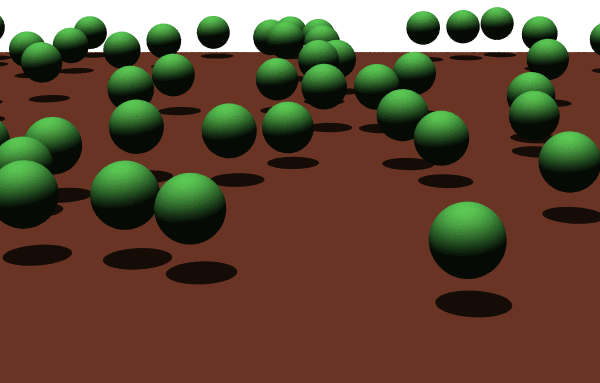
\includegraphics[width=0.33\textwidth]{/home/mn811042/Thesis/chapter4/figures/rami_lai_050.png}}
\subfloat[Medium Canopy]{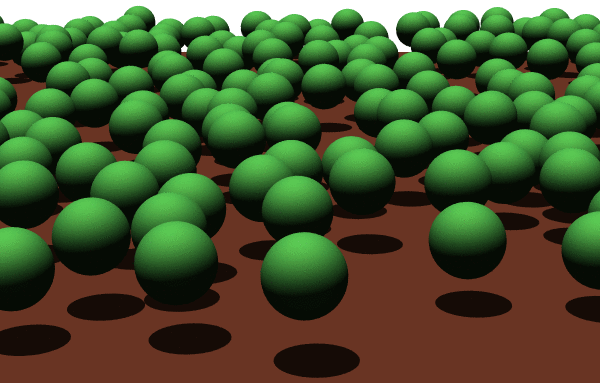
\includegraphics[width=0.33\textwidth]{/home/mn811042/Thesis/chapter4/figures/rami_lai_150.png}}
\subfloat[Dense Canopy]{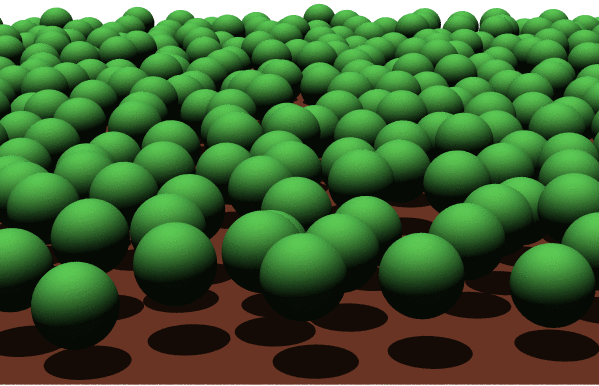
\includegraphics[width=0.33\textwidth]{/home/mn811042/Thesis/chapter4/figures/rami_lai_250.png}}
\end{tabular}
\caption{Graphical representation of the open forest canopy environments used in RAMI4PILPS. The images represent three different canopy structures \citep{Widlowski2011}.} 
\label{fig:rami}
\end{figure}

\subsection{`Clumping indices' vs. 3D model: direct transmissivity}
Direct transmissivities were calculate following Eq.~\ref{equation:pgap} for each one of the different structural variables ($\Omega^{\prime}$s) - $\Omega_e(\theta)$ (\citep{Kucharik1999}), $\gamma$ (\citep{Ni-Meister2010} and $\zeta(\mu)$ (\citep{pinty2006}) (Fig.~\ref{f:ci_comparisons}right).

The 1D case was also calculated following Eq.~\ref{equation:pgap} with $\Omega = 1.0$ and $L_e = LAI$ (\textbf{1D case}).

The 3D tree based model MAESPA (see section~\ref{section:maespa}) was used in the simulations of $P_{gap}(\theta)$ for the RAMI4PILPS scenarios and it was used as the reference model (\textbf{MAESPA}). $P_{gap}(\theta)$ was directly derived from MAESPA by setting a Black Canopy ($\rho_{leaf} = \tau_{leaf} = 0.0$) with different structures and deriving it from fAPAR, as
\begin{equation}
P_{gap} = 1.0 - fAPAR
\label{equation:pgap_black}
\end{equation}

To evaluate the differences between each one of the described parameterisations the RMSE (Root-Mean-Square-Error) was calculated following the equation,
\begin{equation}
RMSE = \sqrt{\frac{\sum_{n=0}^{N} (P_{gap}(\theta)^{\Omega} - P_{gap}(\theta)^{MAESPA})^2}{N}}
\label{equation:rmse_pgap}
\end{equation}
\noindent where N = 85$^{\circ}$ because MAESPA presented numerical instability (e.g. negative values) for the last 5$^{\circ}$ of the complete solar zenith angle range.

\begin{figure}
\centering
\begin{tabular}{ll}
\subfloat[Sparse Canopy]{\includegraphics[width=0.5\textwidth]{/home/mn811042/Thesis/chapter4/figures/CI_comparison_050.png}
                         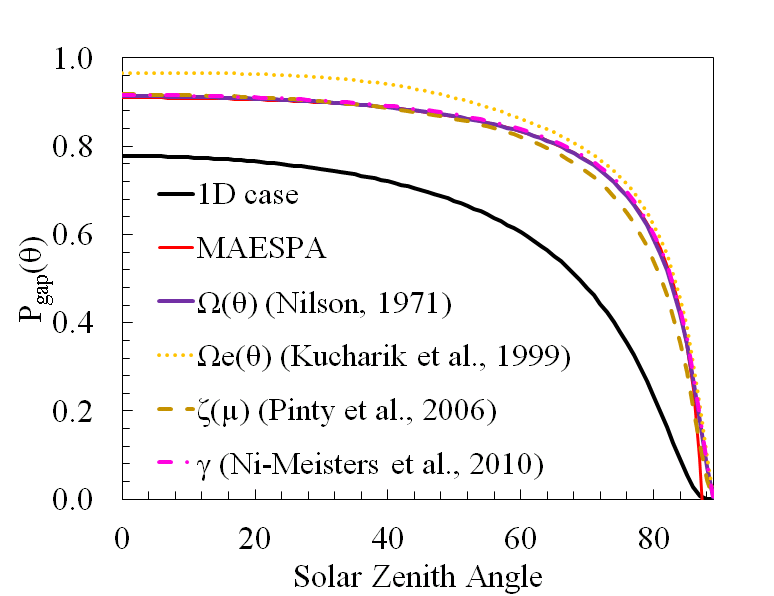
\includegraphics[width=0.5\textwidth]{/home/mn811042/Thesis/chapter4/figures/pgap_comparison_050.png}}
\end{tabular}

\begin{tabular}{ll}
\subfloat[Medium Canopy]{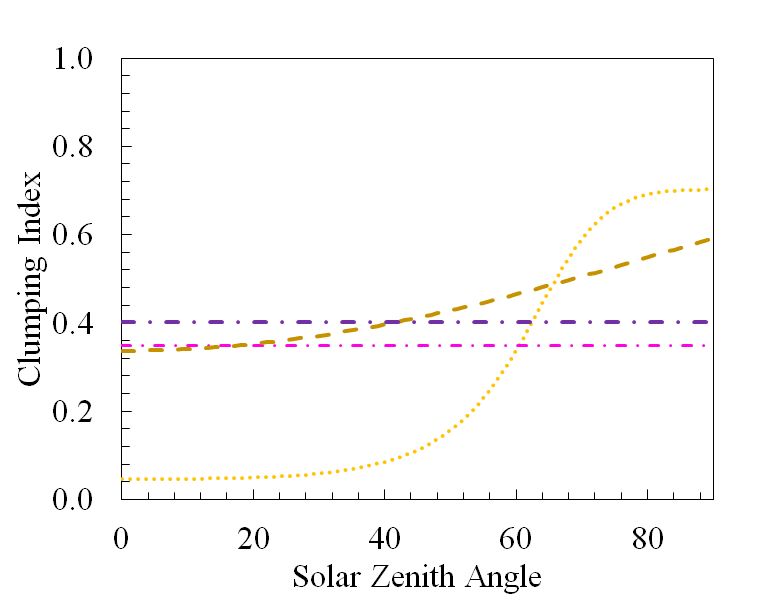
\includegraphics[width=0.5\textwidth]{/home/mn811042/Thesis/chapter4/figures/CI_comparison_150_v2.png}
                         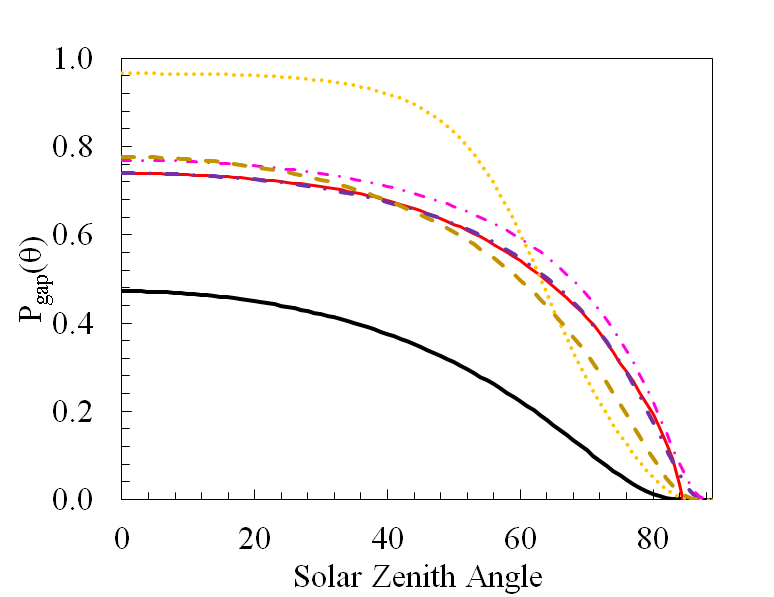
\includegraphics[width=0.5\textwidth]{/home/mn811042/Thesis/chapter4/figures/pgap_comparison_150.png}}
\end{tabular}

\begin{tabular}{ll}
\subfloat[Dense Canopy]{\includegraphics[width=0.5\textwidth]{/home/mn811042/Thesis/chapter4/figures/CI_comparison_250.png}
                        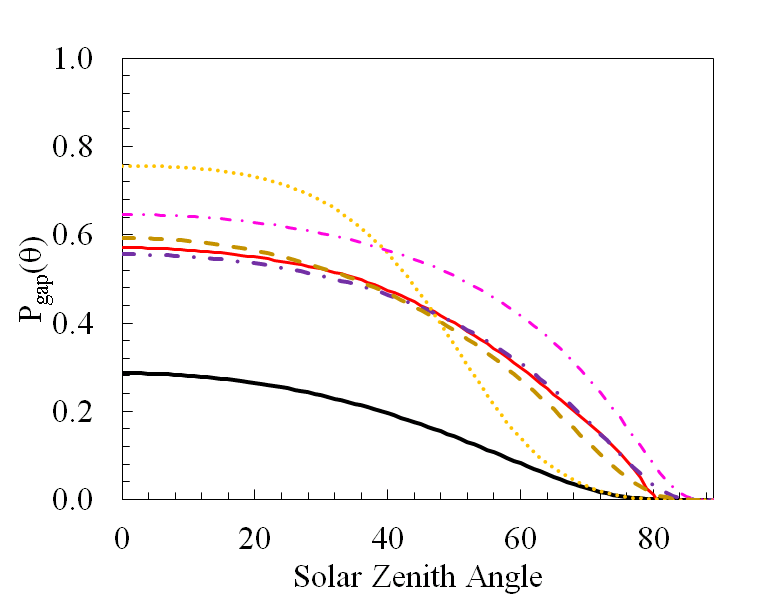
\includegraphics[width=0.5\textwidth]{/home/mn811042/Thesis/chapter4/figures/pgap_comparison_250.png}}
\end{tabular}

\caption{Comparison between different ways to calculate clumping index and its impact on gap fraction.}
\label{f:ci_comparisons}
\end{figure}

By following \citet{Kucharik1999}, it is necessary to know the number of stems within a predetermined ground area, the crown diameter, and the ratio of crown depth to crown diameter. Besides that, this clumping index parameterisation is a semi-empirical equation adjusted for a specific set of data collected in boreal forests during the BOREAS large experiment. Its applicability could not necessarily be extended to other PFTs.

For the sparse canopy, P$_{gap}(\theta)$ obtained with Kucharik$^{\prime}$s method tend to overestimate the reference values by 10\% through the range of evaluated solar zenith angles until about 60$^{\circ}$. For higher solar zenith angles direct transmissivity calculated with this parameterisation agrees well with the reference values obtained with the 3D model.

The first parameterisation presents a clumping index always smaller than the other two for the sparse canopy showing a triple behaviour with a varying zenith angle. From 0$^{\circ}$ to 20$^{\circ}$ the clumping index is approximately constant and equals to 0.15 indicating a large discrepancy between the 1D and the 3D case. From 40$^{\circ}$ to 60$^{\circ}$ the clumping index increases following approximately a linear relationship between solar zenith angle and clumping. After 60$^{\circ}$ the clumping index reaches a second plateau in about 0.35.

Fig.~\ref{fig:ci_rmse} - sparse case indicates that between the three evaluated parameterisations, this one shows larger deviation from the 3D model reference values ($\approx$ 0.15) but still smaller deviation than the 1D case.

For the medium canopy the clumping index also presents the same triple behaviour (plateau - linear relationship - plateau), but at this time with a very distinct behaviour than the other two evaluated parameterisations.

From 0$^{\circ}$ to about 40$^{\circ}$ the clumping index is very small ($\approx$ 0.0), which results in a direct transmissivity of 1.0, or 25\% higher than the 3D reference model. From 40$^{\circ}$ to 70$^{\circ}$, the clumping index presents a rapid increase reaching the second plateau in about P$_{gap}(\theta)$ = 0.7 and underestimates the 3D reference model at the end of the solar zenith angle range.

For the intermediate scenario, this parameterisation showed a performance not as accurate as the other two when compared with the 3D reference model, but still better than the 1D case in average.

In the dense canopy (LAI = 2.5 m$^2$.m$^{-2}$), Kucharik$^{\prime}$s parameterisation behaves only slightly more deviant than the other two in the average by evaluating the RMSE obtained with the 3D model reference values. The behaviour of the clumping index curve with solar zenith angle is about the same than in the other two canopy densities, but with $\Omega(\theta) = 1.0$ at the end of the solar zenith angle range (from 70$^{\circ}$ to 85$^{\circ}$). From this analysis it is possible to say that for this part of the solar zenith range, the evaluated parameterisation gives similar results than the 1D case. Between all three canopy densities, however, to use Kucharik$^{\prime}$s parameterisation results in a smaller error when compared to the reference model, than the 1D case.

While in \citet{Ni-Meister2010}, the relationship for clumping index is based on an analytical prognostic expression, which can also just be determined with previous knowledge about stem density, crown radius and LAI. Besides that, the generalised equation for spheres does not depend on Sun zenith angle and remained constant for the evaluated scenarios ($\gamma \approx 0.35$).

The variable that determines the clumping index from \citet{Ni-Meister2010} is $\tau_0r$, which is proportional to LAI and $\lambda$ (see Eq.~\ref{equation:clumpNi} for reference). For the RAMI4PILPS scenarios LAI and $\lambda$ increase at the same proportion and as a result the clumping index for all the three scenes was kept constant, but without greatly compromising the final P$_{gap}(\theta)$. In the average, Ni-Meister$^{\prime}$s clumping index fairly agreed with the reference model for all evaluated scenarios.

For all evaluated cases, Ni-Meister$^{\prime}$s parameterisation showed a better agreement with the reference model than the 1D case, and especifically for the medium case, this parameterisation presented better results (smaller RMSE) than all the the other parameterisations evaluated.  

For the dense case, Ni-Meister$^{\prime}$s parameterisation overestimate P$_{gap}(\theta)$ reference along all solar zenith angles in about 10\%, by considering the canopy `gappier' than it actually was. However, overall this parameterisation seemed to give similar results than the 3D model reference values. 

By using the structure factor parameterisation \citep{pinty2006}, there is no need to have previous knowledge about canopy structure, whereas the parameters are minimised against terms of the radiation partitioning (absorbance, reflectance and transmittance), either measured, or calculated by detailed radiative transfer schemes (see Section~\ref{sub:minimise}). Overall, the structure factor presented the better agreement with the 3D model reference values of P$_{gap}(\theta)$.

For the sparse and medium cases, the structure factor was of the same order than the clumping index of \citet{Ni-Meister2010} for small solar zenith angles, e.g. smaller than 40$^{\circ}$ for the sparse case and smaller than 20$^{\circ}$ for the medium case. The difference however is on the fact that the structure factor increases with solar zenith angle, which is equivalent to say that the radiation path length gets larger a lower Sun in the sky. 

By comparing the gap probability generated with three different parameterisations with the one generated by the MAESPA model, the structure factor presented the lowest averaged RMSE (Fig.~\ref{fig:ci_rmse}) and because of that, only this parameterisation will be used in further evaluations. Results are summarised in Fig.~\ref{f:ci_comparisons}(left).

\begin{figure}
\centering
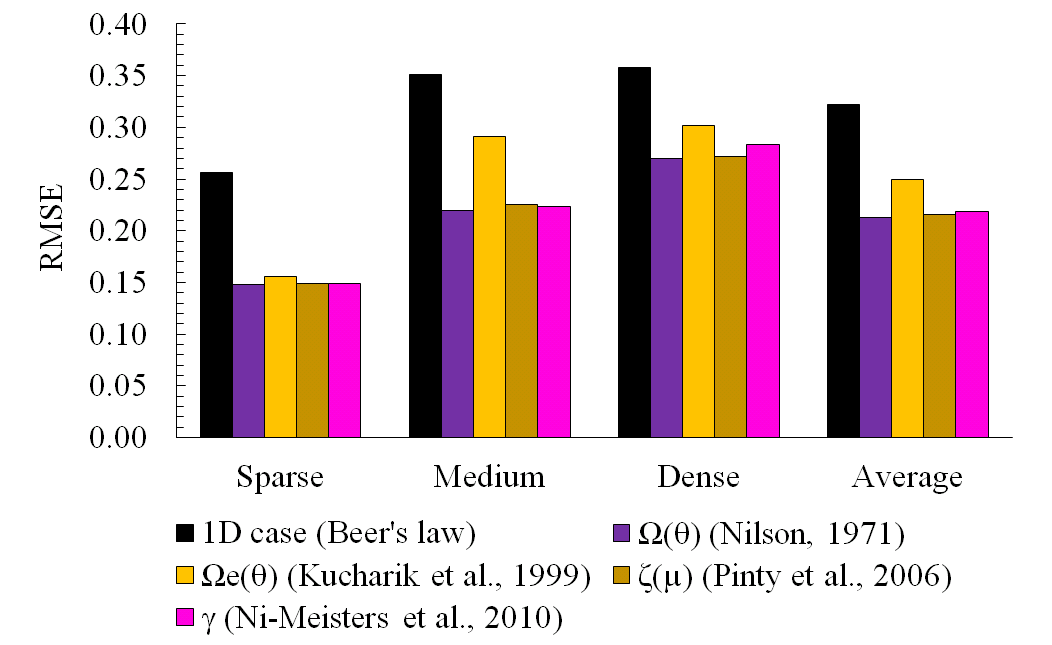
\includegraphics[width=1.0\textwidth]{/home/mn811042/Thesis/chapter4/figures/CI_rmse_v2.png}
\caption{Root-Mean-Squared-Error of gap probability generated with three structural parameterisations and MAESPA for three different canopies densities (sparse, medium and dense) and the average.} 
\label{fig:ci_rmse}
\end{figure}

\subsection{Impacts of the structure factor parameterisation on direct transmissivity}
The structure factor is described by a linear combination of two distinct elements $a$ and $b$ as discussed before, but what are the differences caused by theses different elements on the radiation partitioning?

In order to look at the impact of each one of these two elements on direct transmissivity the Eq.~\ref{equation:pgap} was used for each one the canopy densities described in Table~\ref{tab:RAMI4PILPS} and represented by Fig.~\ref{fig:rami}. The `clumping index' ($\Omega$) in here referred as `structure factor' ($\zeta(\mu)$) is described by Eq.~\ref{equation:structurefactor} and the multiple zenith variations were summed over 90$^{\circ}$ following the equation bellow, 
\begin{equation}
P_{gap}^{ab} = \sqrt{\frac{\sum_{\theta=0^{\circ}}^{N} (P_{gap}(\theta))^2}{N}}
\label{equation:pgapab}
\end{equation}
\noindent where N = 90$^{\circ}$ and both elements $a$ and $b$ varied from 0.0 to 1.0. 

Figure~\ref{f:pgap_ab} shows the impact of $a$ and $b$ combined on direct transmissivity. Both parameters affect $P_{gap}(\theta)$ on a relative similar way, but with strong dependency on canopy density. For example, when the parameters values are close to 0.0, the direct transmissivity is increased, because the `structure factor' acts on the way to reduce the total optical depth of the canopy. 

On the other hand, by increasing both parameters, the direct transmissivity is reduced. If $a$ = $b$ = 1, the `effective' optical depth is equivalent to twice the true LAI ($L_e = LAI \cdot [1.0 + 1.0 (1 - cos(90^{\circ})] = 2 \cdot LAI$).

It is also possible to notice that the impact of $b$ decreases with canopy density. For the sparse canopy the variation of $P_{gap}(\theta)$ with $a$ and $b$ is almost the same, once the largest gradient in Fig~\ref{f:pgap_ab} is oblique to both axis. 

The dense canopy, however, shows a larger variation of $P_{gap}(\theta)$ parallel to the x-axis, which means $a$ has a greater impact on direct transmissivity. The medium canopy presents a intermediate behaviour with $a$ being more impacting than $b$ on $P_{gap}(\theta)$.

The results presented in this section suggest the importance of considering solar zenith angular variations for sparse canopies with relative low LAI.

\begin{figure}
\centering
\begin{tabular}{lll}
\subfloat[Sparse]{\includegraphics[width=0.33\textwidth]{/home/mn811042/src/julesRT_struct/Pgap_matrix_a_b_050_v2.png}}
\subfloat[Medium]{\includegraphics[width=0.33\textwidth]{/home/mn811042/src/julesRT_struct/Pgap_matrix_a_b_150_v2.png}}
\subfloat[Dense]{\includegraphics[width=0.33\textwidth]{/home/mn811042/src/julesRT_struct/Pgap_matrix_a_b_250_v2.png}}
\end{tabular}
\caption{P$_{gap}$ calculated over all possible solar zenith angles with the modified Two-stream scheme with the structure factor varying $a$ and $b$ from 0 to 1 for three canopies densities (sparse, medium and dense).}
\label{f:pgap_ab}
\end{figure}

\subsection{Angular impacts of the structure factor parameters on absorption}\label{sub:angular}
It is possible to determine the relative influence of both structure factor parameters $a$ and $b$ independently for different solar zenith angles (Fig.~\ref{f:fapar_ab}).

Because $b$ is a parameter that modulates angular variation as represented in Eq.~\ref{equation:structurefactor}, it is expect a more effective impact of $b$ on radiative transfer calculations for larger Sun zenith angles.

\begin{figure}[ht!]
\centering
\begin{tabular}{lll}
\subfloat[Sparse]{\includegraphics[width=0.33\textwidth]{/home/mn811042/src/julesRT_struct/fAPAR_matrix_a_b_lai_050_sza_27_big_2.png}
\includegraphics[width=0.33\textwidth]{/home/mn811042/src/julesRT_struct/fAPAR_matrix_a_b_lai_050_sza_60_big_2.png}
\includegraphics[width=0.33\textwidth]{/home/mn811042/src/julesRT_struct/fAPAR_matrix_a_b_lai_050_sza_83_big_2.png}}
\end{tabular}

\begin{tabular}{lll}
\subfloat[Medium]{\includegraphics[width=0.33\textwidth]{/home/mn811042/src/julesRT_struct/fAPAR_matrix_a_b_lai_150_sza_27_big_2.png}
                 \includegraphics[width=0.33\textwidth]{/home/mn811042/src/julesRT_struct/fAPAR_matrix_a_b_lai_150_sza_60_big_2.png}
                 \includegraphics[width=0.33\textwidth]{/home/mn811042/src/julesRT_struct/fAPAR_matrix_a_b_lai_150_sza_83_big_2.png}}
\end{tabular}

\begin{tabular}{lll}
\subfloat[Dense]{\includegraphics[width=0.33\textwidth]{/home/mn811042/src/julesRT_struct/fAPAR_matrix_a_b_lai_250_sza_27_big_2.png}
                 \includegraphics[width=0.33\textwidth]{/home/mn811042/src/julesRT_struct/fAPAR_matrix_a_b_lai_250_sza_60_big_2.png}
                 \includegraphics[width=0.33\textwidth]{/home/mn811042/src/julesRT_struct/fAPAR_matrix_a_b_lai_250_sza_83_big_2.png}}
\end{tabular}
\caption{Sensitivity analysis of fAPAR for a range of structure factor parameters $a$ and $b$ varying from 0.0 to 1.0, for a set of three different canopy densities and three sun zenith angles (see Table~\ref{tab:RAMI4PILPS}).}
\label{f:fapar_ab}
\end{figure}

A more rapid variation of fAPAR associate with a sun zenith angle of 27.5$^{\circ}$ following values of parameter $a$ on the x-axis indicates a relative larger impact of that variable than the one caused by the parameter $b$. Also, it is possible to conclude that a higher LAI is responsible for larger variations of fAPAR with the parameter $a$, represented by a more distinguishable variation in colours (Fig.~\ref{f:fapar_ab}). 

For larger Sun zenith angles (60.0$^{\circ}$ and 83.5$^{\circ}$) the inclination of lines intervals towards the $b$ parameter becomes steeper, which indicates an increase of the impact of parameter $b$ on the final result of fAPAR. 

\section{Evaluating the `Structure Factor' Radiation Partitioning: Zenith Profile}
This section will use six different radiative transfer approaches to obtain the zenith profile of radiation partitioning for the RAMI4PILPS scenes. The RAMI4PILPS reference values were calculated through a Monte Carlo approach and is referred as \textbf{RAMI4PILPS}. Two of the radiative transfer schemes, \textbf{GORT} \citep{Li1995,Ni1997} and \textbf{MAESPA} \citep{Wang1990,Medlyn2004,Medlyn2007} are 3D models that use different radiative transfer theories to describe sparsely vegetated canopies. 

The 1D radiative transfer scheme used in here is the Two-Stream approximation \citep{Sellers1985}, which is widely used in GCMs, and it was isolated from the main body of the JULES code \citep{Best2011,Clark2011} and because of that it is referred as \textbf{JULES}.
Also, in order to evaluate an approach often implemented in GCMs to account for sparse vegetated canopies, a commonly used `correction' based on the amount of vegetation cover on a model grid cell is applied, referred as \textbf{JULES$_{VegFraction}$}. 
Finally, the `structure factor' parameterisation \citep{pinty2006} was implemented in the Two-Stream radiative transfer version in JULES and is referred as \textbf{JULES$_{Structure}$}. 

\subsection{MAESTRA/MAESPA}\label{section:maespa}
The MAESTRA/MAESPA model \citep{Wang1990,Medlyn2004,Medlyn2007,Duursma2012} represents a forest canopy as an array of tree crowns, whose positions and dimensions are specified. The radiation routines are described in detail by \citet{Wang1990}. The canopy consists of individual tree crowns, which are described by a basic shape (one of several shapes, including ellipsoids, cylinders and cones), length, height to crown base, and width (in x and y directions). Radiation calculations are performed only for a set of target crowns specified by the user. The distribution of leaf area within the target crown is specified, as is the leaf angle distribution. The target crown is divided into usually 60 grid points, and the radiation penetrating to each grid point is calculated for three wavebands (PAR, NIR and thermal infra-red, TIR) based on shading within the crown, shading by neighbouring trees, the location of the sun, and whether radiation is direct or diffuse. Direct, diffuse and scattered radiation are considered separately. Scattering of radiation is approximated following \citet{Norman1979}. Leaf area within crowns is assumed to be distributed randomly \citep{Wang1990}. At each grid point, leaf area is separated into sunlit and shaded leaf area (Norman, 1993). The model has previously been applied to study canopy carbon and water fluxes of \textit{Picea sitchensis} \citep{Wang1990}, \textit{Pinus radiata} \citep{McMurtrie1993}, \textit{Betula pendula} \citep{Wang1998}, and \textit{Pinus taeda} \citep{Luo2001}. 
%Using the $R$ (R Development Core Team, 2011) package, Maeswrap (Duursma, 2015), the 3D stand scenes were graphically reproduced in 3D.

\subsection{GORT} 
The GORT model was developed to describe the effects of three-dimensional canopy structure on the radiation environment and to characterise the heterogeneous radiation environment in natural vegetation at the forest stand scale \citep{Li1995}. Merging theory from geometric optics and radiative transfer, the GORT model treats vegetation canopies as assemblages of randomly distributed tree crowns of ellipsoidal shape. The tree crowns are filled with leaves that absorb and scatter radiation passing through the crown. Principles of radiative transfer are used in describing the multiple scattering of leaves inside crowns and the multiple scattering among crowns and the ground surface. The GORT model was extended by \citet{Ni1997} to include the vertical canopy gap probability profile. For this exercise the PAR radiation spectrum was centred in 550 nm, and NIR in 850 nm.

\subsection{Two-Stream: JULES (the Joint UK Land Environment Simulator)} 
The Two-Stream scheme assumes that diffuse radiative fluxes are isotropic in the upward and downward directions. Supposing that the upper and lower leaf optical properties are identical, the Two-Stream scheme used to model radiative transfer in plant canopies is given in the following form \citep{Dickinson1983,Sellers1985}: 
\begin{equation}
\begin{gathered}
-\overline{\mu}(dI^{\uparrow})/dL + [1 - (1 - \beta)\omega]I^{\uparrow} - \omega \beta I^{\downarrow} = \omega \overline{\mu} K \beta_0 \exp{(-KL)},\\
-\overline{\mu}(dI^{\downarrow})/dL + [1 - (1 - \beta)\omega]I^{\downarrow} - \omega \beta I^{\uparrow} = \omega \overline{\mu} K (1-\beta_0) \exp{(-KL)}
\end{gathered}
\label{equation:ts}
\end{equation}
\noindent where $I^{\uparrow}$ and $I^{\downarrow}$ are the upward and downward diffuse radiative fluxes normalized by the incident flux respectively, $\mu$ is the cosine of the zenith angle of the incident beam, $K$ is the optical depth of direct beam per unit leaf area and is equal to $G(\mu)/\mu$, $G(\mu)$ is the relative projected area of leaf elements in the direction $cos^{-1}\mu$, $\overline{\mu}$ is the average inverse diffuse optical depth per unit leaf area and is equal to $\int_{0}^{1}[\mu^{\prime}/G(\mu^{\prime})]d\mu^{\prime}$, $\mu^{\prime}$ is the direction of scattered flux, $\omega$ is the scattering coefficient and is equal to $\rho_{leaf} + \tau_{leaf}$, and $L$ is the cumulative LAI. $\beta$ and $\beta_0$ are upscattering parameters for the diffuse and direct beams respectively (see \citet{Sellers1985} for details). 

The version used in this exercise was extracted from the JULES model. The JULES model is the UK community land surface model designed to be interfaced with the UK Met Office Unified Model \citep{Walters2014} by predicting fluxes of heat, water and carbon between the land surface and the atmosphere. It originates from the Met Office Surface Exchange Scheme (MOSES) \citep{Cox1999}, and it includes the TRIFFID (Top-down Representation of Interactive Foliage and Flora Including Dynamics) dynamic vegetation model \citep{Cox2001}. The physical basis of JULES is common to most of the land surface models and are described in details in \citet{Best2011} and \citet{Clark2011}.

JULES uses a number of layers (10 in this exercise) with equally distributed LAI to calculate the radiative transfer in the canopy for direct and diffuse radiation separately. The leaves extinction properties are prescribed by leaf reflectance ($\rho_{leaf}$) and transmittance ($\tau_{leaf}$) in the PAR and NIR wavebands and canopy leaf angle distribution (spherical or horizontal). The amount of absorbed incident radiation at each layer is therefore determined by sun zenith angle, incident direct and diffuse radiation at the top of the canopy, and the leaves extinction coefficients. 

\subsection{Vegetation cover approach}
More simplified approaches to handle sparse vegetated canopies have been implemented in GCMs and are widely used \citep{Loew2014}. The vegetation cover approach is one of them and it is described bellow.

Suppose a model grid cell with area $A$, which is assumed to be fully covered (100\%) by a particular plant functional type (PFT). In the case of sparser canopies like, e.g., savannahs, the area $A$ is covered by a dominant PFT (usually taller trees), a second PFT, for example, understory vegetation (e.g. shrubs, grass), or bare soil. The total area $A$ is thus defined as,
\begin{equation}
A = Veg_{fraction} + Under_{fraction}
\label{equation:area}
\end{equation}
\noindent where $Veg_{fraction}$ is the fractional coverage of the major PFT and $Under_{fraction}$ corresponds to to the soil surface.  If the $LAI_{total}$ is the LAI over the area A, the LAI correspondent to the area $Veg_{fraction}$ is given by,
\begin{equation}
LAI_{Veg_{fraction}} = \frac{LAI_{Total}}{Veg_{fraction}}
\label{equation:laivegfraction}
\end{equation}
\noindent where $LAI_{Veg_{fraction}} \geq LAI_{Total}$. The correspondent fAPAR to the new area can be calculated as, 
\begin{equation}
fAPAR_{Veg_{fraction}} = fAPAR(LAI_{Veg_{fraction}})\cdot Veg_{fraction}
\label{equation:faparvegfraction}
\end{equation}
\noindent where fAPAR(LAI$_{Veg}_{fraction}$) is the `new' fAPAR calculated with the Two-Stream scheme using LAI$_{Veg}_{fraction}$. 

And the correspondent canopy albedo ($\alpha_{Veg}_{fraction}$) can be obtained as, 
\begin{equation}
\alpha_{Veg_{fraction}} = (\alpha_{canopy}(LAI_{Veg_{fraction}}) \cdot Veg_{fraction} + (1 - Veg_{fraction}) \cdot \alpha_{soil})
\label{equation:albedovegfraction}
\end{equation}
\noindent where $\alpha_{canopy}$ is the `new' canopy albedo calculated with the Two-Stream scheme using LAI$_{Veg}_{fraction}$. 

\subsection{Solar Zenith Angular evaluations}
This section shows the results for absorption and reflectance in the PAR and NIR spectral regions obtained with six radiative transfer approaches represented in Figures~\ref{f:szacomparisonfPAR},\ref{f:szacomparisonalbPAR},\ref{f:szacomparisonfNIR} and \ref{f:szacomparisonalbNIR}.

The Two-Stream scheme, referred in the figures as \textbf{JULES} overestimates the reference values for PAR absorption over all evaluated canopy densities under both illumination conditions. This behaviour indicates that this scheme is more optically opaque for PAR radiation than the 3D Monte Carlo reference model due to architectural features. 

For PAR reflectance, the Two-Stream scheme underestimates the reference values over the majority of evaluated canopy densities under both illumination conditions, except over black soil albedo. In this case, the Two-Stream scheme reflects more PAR radiation from the plant elements, because it does not `see' the underneath  black soil as much as the other schemes, that take structural variabilities into account.

In the NIR spectrum the Two-Stream scheme presents a relative agreement with the reference values for absorption, especially in solar zenith angles equals 60$^{\circ}$ and under diffuse illumination condition. For the other cases, the Two-Stream scheme tends to overestimate the reference values for small solar zenith angles ($\approx$ 27.5$^{\circ}$) and the opposite for high solar zenith angles ($\approx$ 83.5$^{\circ}$).

For canopy reflectance, the Two-Stream scheme tends to overestimate it over small soil albedos (black and medium) and show relative agreement over bright soil (snow).

MAESPA seems to be an efficient tool to calculate PAR absorption for different vegetation canopies, as it strongly agreed with the RAMI4PILPS reference values for PAR absorption, especially over non-bright surfaces. Over bright surfaces (snow), MAESPA values underestimate the reference values, which indicates some sort of misrepresentation of soil reflectance into the vegetation canopy.

In the NIR spectrum MAESPA was able to reproduce the shape of the curve associated with absorption, but underestimating the reference values in up to 10\% in a dense canopy over snow. The results of reflectance were not generated with the MAESPA model.

Also evaluated in this study, the GORT model was developed to describe the effects of 3D canopy structure on reflectance in natural vegetation at the forest stand scale \citep{Ni1999}. The description of canopy structure in GORT is statistical, i.e., with minimum and maximum values of tree height, crown radius and tree density. The GORT model was also considered in this experiment, because it calculates albedo values, which are not directly obtained from MAESPA.

In the PAR spectrum GORT presented high agreement with the RAMI4PILPS reference values for the sparse case scenario over all soil reflectances for direct illumination in the solar zenith angle range going from 0$^{\circ}$ to 60$^{\circ}$. For higher solar zenith angles, GORT underestimates PAR absorption up to 20\% over a black soil ($\alpha_{soil}$ = 0.0) background. For diffuse illumination the GORT model agrees with the reference values. 

As the canopy density increases PAR absorption generated by the GORT model starts to be underestimated, especially over snow ($\alpha_{soil}$ = 0.96), for direct and diffuse illumination conditions.

For PAR reflectance, GORT underestimates the reference values over black soil for all the evaluated canopy densities. For the medium soil albedo, GORT seemed to be the model which agreed most with the reference values, especially over the medium canopy, GORT was able to characterise exactly the decay of PAR reflectance following solar zenith angles. Over snow, GORT tends to overestimate PAR reflectance, especially over the dense canopy.   

In the NIR spectrum GORT presented a persistent overestimation in absorption and underestimation in reflectance for both illumination conditions. Moreover, GORT was not able to reproduce the increasing curve of NIR reflectance in all evaluated cases.

Also presented in this comparison study, JULES$_{VegFraction}$, the vegetation fraction `correction', is a common approach applied to account for canopy gaps in operational radiative balance calculations. \citet{Loew2014} applied the correction by simply multiplying the fAPAR by the fraction of vegetation cover, however it was assumed here that the more appropriate way to do it is by: first, calculating the fAPAR for the `concentrated LAI' in a smaller area, which is the LAI divided by the fraction of vegetation cover. After that, with the correct LAI, the fAPAR is calculated with the new value, and the correction is proceeded by multiplying the new fAPAR by the fraction of vegetation cover (Eq.~\ref{equation:faparvegfraction}). 

This 1D correction reproduces the absorbance and reflectance of more complex models for low Sun zenith angles ($< 30^{\circ}$) and non-reflective backgrounds ($\alpha_{soil} \approx 0.0$), but does not reproduce the complete angular variation associated with variables used to obtain the radiative balance. This approach was able to reproduce the canopy reflectance comparable to the reference values for all canopy densities over black soil better than any other scheme. Over brighter soils (medium and snow), however this approach can overestimate the reference values up to 25\% over dense canopies with snow. This approach is limited to account for multiple scattering because it uses the same Two-Stream with a larger LAI.  

Figures~\ref{f:szacomparisonfPAR} indicates that overall, JULES$_{Structure}$ (red dashed line) consistently showed a better agreement to the RAMI4PILPS reference values (black crosses) than any other approach under direct (Solar Zenith Angles from 0 to 90$^{\circ}$) and diffuse illumination (ISO stands for isotropic) conditions. It seemed to be an efficient and accurate tool to derive PAR absorbance and reflectance for all evaluated scenarios, with especial attention to its performance over brighter backgrounds (snow). 

This effect is particularly relevant for the radiative balance treatment in boreal regions in the presence of snow, where the shadowing induced by spatially distributed plant structures diminishes surface albedo in comparison with a closed-canopy/bare-snow scenario of identical cover fractions \citep{Viterbo1999}. JULES$_{Structure}$ presented a better agreement with the reference values than any other model for absorbance and reflectance over snow. 

In the NIR spectrum, the structure factor improves the agreement between Two-Stream scheme and the RAMI4PILPS reference values in the sparse canopy for absorption and reflectance, but has the opposite effect over the other canopy densities. In particular over bright soils the structure factor improves the agreement for absorption, but it is not capable to reproduce the reference values associated with high solar zenith angles at the end of the range ($83.5^{\circ}$).

The next section explores in details the differences between the Two-Stream and the parameterised Two-Stream with the structure factor in relation to the RAMI4PILPS reference values.

\begin{figure}
\centering
\begin{tabular}{lll}
\subfloat[Sparse]{\includegraphics[width=0.33\textwidth]{/home/mn811042/src/julesRT_struct_2/julesRT_struct/JULES_STRUCT_FACTOR/fabs_PAR_050_BLK_STRUC.png}
                  \includegraphics[width=0.33\textwidth]{/home/mn811042/src/julesRT_struct_2/julesRT_struct/JULES_STRUCT_FACTOR/fabs_PAR_050_MED_STRUC.png}
                  \includegraphics[width=0.33\textwidth]{/home/mn811042/src/julesRT_struct_2/julesRT_struct/JULES_STRUCT_FACTOR/fabs_PAR_050_SNW_STRUC.png}}
\end{tabular}
\begin{tabular}{lll}
\subfloat[Medium]{\includegraphics[width=0.33\textwidth]{/home/mn811042/src/julesRT_struct_2/julesRT_struct/JULES_STRUCT_FACTOR/fabs_PAR_150_BLK_STRUC.png}
                  \includegraphics[width=0.33\textwidth]{/home/mn811042/src/julesRT_struct_2/julesRT_struct/JULES_STRUCT_FACTOR/fabs_PAR_150_MED_STRUC.png}
                  \includegraphics[width=0.33\textwidth]{/home/mn811042/src/julesRT_struct_2/julesRT_struct/JULES_STRUCT_FACTOR/fabs_PAR_150_SNW_STRUC.png}}
\end{tabular}
\begin{tabular}{lll}
\subfloat[Dense]{\includegraphics[width=0.33\textwidth]{/home/mn811042/src/julesRT_struct_2/julesRT_struct/JULES_STRUCT_FACTOR/fabs_PAR_250_BLK_STRUC.png}
                 \includegraphics[width=0.33\textwidth]{/home/mn811042/src/julesRT_struct_2/julesRT_struct/JULES_STRUCT_FACTOR/fabs_PAR_250_MED_STRUC.png}
                 \includegraphics[width=0.33\textwidth]{/home/mn811042/src/julesRT_struct_2/julesRT_struct/JULES_STRUCT_FACTOR/fabs_PAR_250_SNW_STRUC.png}}
\end{tabular}
\caption{Solar zenith profile of fraction of direct and diffuse (ISO) absorbed PAR calculated with 6 different models. JULES$_{Structure}$ parameters were obtained for each canopy density through inversion of fAPAR and albedo PAR values together over three soil backgrounds (BLK = black, $\alpha_{soil}$ = 0.00; MED = medium, $\alpha_{soil}$ = 0.12; and SNW = snow, $\alpha_{soil}$= 0.96). The obtained values of each structure factor parameters are described in Table~\ref{tab:structureparameters}.}
\label{f:szacomparisonfPAR}
\end{figure}

\begin{figure}
\centering
\begin{tabular}{lll}
\subfloat[Sparse]{\includegraphics[width=0.33\textwidth]{/home/mn811042/src/julesRT_struct_2/julesRT_struct/JULES_STRUCT_FACTOR/fref_PAR_050_BLK_STRUC.png}
                  \includegraphics[width=0.33\textwidth]{/home/mn811042/src/julesRT_struct_2/julesRT_struct/JULES_STRUCT_FACTOR/fref_PAR_050_MED_STRUC.png}
                  \includegraphics[width=0.33\textwidth]{/home/mn811042/src/julesRT_struct_2/julesRT_struct/JULES_STRUCT_FACTOR/fref_PAR_050_SNW_STRUC.png}}
\end{tabular}
\begin{tabular}{lll}
\subfloat[Medium]{\includegraphics[width=0.33\textwidth]{/home/mn811042/src/julesRT_struct_2/julesRT_struct/JULES_STRUCT_FACTOR/fref_PAR_150_BLK_STRUC.png}
                  \includegraphics[width=0.33\textwidth]{/home/mn811042/src/julesRT_struct_2/julesRT_struct/JULES_STRUCT_FACTOR/fref_PAR_150_MED_STRUC.png}
                  \includegraphics[width=0.33\textwidth]{/home/mn811042/src/julesRT_struct_2/julesRT_struct/JULES_STRUCT_FACTOR/fref_PAR_150_SNW_STRUC.png}}
\end{tabular}

\begin{tabular}{lll}
\subfloat[Dense]{\includegraphics[width=0.33\textwidth]{/home/mn811042/src/julesRT_struct_2/julesRT_struct/JULES_STRUCT_FACTOR/fref_PAR_250_BLK_STRUC.png}
                 \includegraphics[width=0.33\textwidth]{/home/mn811042/src/julesRT_struct_2/julesRT_struct/JULES_STRUCT_FACTOR/fref_PAR_250_MED_STRUC.png}
                 \includegraphics[width=0.33\textwidth]{/home/mn811042/src/julesRT_struct_2/julesRT_struct/JULES_STRUCT_FACTOR/fref_PAR_250_SNW_STRUC.png}}
\end{tabular}
\caption{Solar zenith profile of fraction of direct and diffuse (ISO) reflected PAR calculated with 6 different models. JULES$_{Structure}$ parameters were obtained for each canopy density through inversion of fAPAR and albedo PAR values together over three soil backgrounds (BLK = black, $\alpha_{soil}$ = 0.00; MED = medium, $\alpha_{soil}$ = 0.12; and SNW = snow, $\alpha_{soil}$= 0.96). The obtained values of each structure factor parameters are described in Table~\ref{tab:structureparameters}.}
\label{f:szacomparisonalbPAR}
\end{figure}

\begin{figure}
\centering
\begin{tabular}{lll}
\subfloat[Sparse]{\includegraphics[width=0.33\textwidth]{/home/mn811042/src/julesRT_struct_2/julesRT_struct/JULES_STRUCT_FACTOR/fabs_NIR_050_BLK_STRUC_pysellers.png}
                  \includegraphics[width=0.33\textwidth]{/home/mn811042/src/julesRT_struct_2/julesRT_struct/JULES_STRUCT_FACTOR/fabs_NIR_050_MED_STRUC_pysellers.png}
                  \includegraphics[width=0.33\textwidth]{/home/mn811042/src/julesRT_struct_2/julesRT_struct/JULES_STRUCT_FACTOR/fabs_NIR_050_SNW_STRUC_pysellers.png}}
\end{tabular}
\begin{tabular}{lll}
\subfloat[Medium]{\includegraphics[width=0.33\textwidth]{/home/mn811042/src/julesRT_struct_2/julesRT_struct/JULES_STRUCT_FACTOR/fabs_NIR_150_BLK_STRUC_pysellers.png}
                  \includegraphics[width=0.33\textwidth]{/home/mn811042/src/julesRT_struct_2/julesRT_struct/JULES_STRUCT_FACTOR/fabs_NIR_150_MED_STRUC_pysellers.png}
                  \includegraphics[width=0.33\textwidth]{/home/mn811042/src/julesRT_struct_2/julesRT_struct/JULES_STRUCT_FACTOR/fabs_NIR_150_SNW_STRUC_pysellers.png}}
\end{tabular}
\begin{tabular}{lll}
\subfloat[Dense]{\includegraphics[width=0.33\textwidth]{/home/mn811042/src/julesRT_struct_2/julesRT_struct/JULES_STRUCT_FACTOR/fabs_NIR_250_BLK_STRUC_pysellers.png}
                 \includegraphics[width=0.33\textwidth]{/home/mn811042/src/julesRT_struct_2/julesRT_struct/JULES_STRUCT_FACTOR/fabs_NIR_250_MED_STRUC_pysellers.png}
                 \includegraphics[width=0.33\textwidth]{/home/mn811042/src/julesRT_struct_2/julesRT_struct/JULES_STRUCT_FACTOR/fabs_NIR_250_SNW_STRUC_pysellers.png}}
\end{tabular}
\caption{Solar zenith profile of fraction of direct and diffuse (ISO) absorbed NIR calculated with 6 different models. JULES$_{Structure}$ parameters were obtained for each canopy density through inversion of fAPAR and albedo PAR values together over three soil backgrounds (BLK = black, $\alpha_{soil}$ = 0.00; MED = medium, $\alpha_{soil}$ = 0.12; and SNW = snow, $\alpha_{soil}$= 0.96). The obtained values of each structure factor parameters are described in Table~\ref{tab:structureparameters}.}
\label{f:szacomparisonfNIR}
\end{figure}

\begin{figure}
\centering
\begin{tabular}{lll}
\subfloat[Sparse]{\includegraphics[width=0.33\textwidth]{/home/mn811042/src/julesRT_struct_2/julesRT_struct/JULES_STRUCT_FACTOR/fref_NIR_050_BLK_STRUC_pysellers.png}
                  \includegraphics[width=0.33\textwidth]{/home/mn811042/src/julesRT_struct_2/julesRT_struct/JULES_STRUCT_FACTOR/fref_NIR_050_MED_STRUC_pysellers.png}
                  \includegraphics[width=0.33\textwidth]{/home/mn811042/src/julesRT_struct_2/julesRT_struct/JULES_STRUCT_FACTOR/fref_NIR_050_SNW_STRUC_pysellers.png}}
\end{tabular}
\begin{tabular}{lll}
\subfloat[Medium]{\includegraphics[width=0.33\textwidth]{/home/mn811042/src/julesRT_struct_2/julesRT_struct/JULES_STRUCT_FACTOR/fref_NIR_150_BLK_STRUC_pysellers.png}
                  \includegraphics[width=0.33\textwidth]{/home/mn811042/src/julesRT_struct_2/julesRT_struct/JULES_STRUCT_FACTOR/fref_NIR_150_MED_STRUC_pysellers.png}
                  \includegraphics[width=0.33\textwidth]{/home/mn811042/src/julesRT_struct_2/julesRT_struct/JULES_STRUCT_FACTOR/fref_NIR_150_SNW_STRUC_pysellers.png}}
\end{tabular}
\begin{tabular}{lll}
\subfloat[Dense]{\includegraphics[width=0.33\textwidth]{/home/mn811042/src/julesRT_struct_2/julesRT_struct/JULES_STRUCT_FACTOR/fref_NIR_250_BLK_STRUC_pysellers.png}
                 \includegraphics[width=0.33\textwidth]{/home/mn811042/src/julesRT_struct_2/julesRT_struct/JULES_STRUCT_FACTOR/fref_NIR_250_MED_STRUC_pysellers.png}
                 \includegraphics[width=0.33\textwidth]{/home/mn811042/src/julesRT_struct_2/julesRT_struct/JULES_STRUCT_FACTOR/fref_NIR_250_SNW_STRUC_pysellers.png}}
\end{tabular}
\caption{Solar zenith profile of fraction of direct and diffuse (ISO) reflected NIR calculated with 6 different models. JULES$_{Structure}$ parameters were obtained for each canopy density through inversion of fAPAR and albedo PAR values together over three soil backgrounds (BLK = black, $\alpha_{soil}$ = 0.00; MED = medium, $\alpha_{soil}$ = 0.12; and SNW = snow, $\alpha_{soil}$= 0.96). The obtained values of each structure factor parameters are described in Table~\ref{tab:structureparameters}.}
\label{f:szacomparisonalbNIR}
\end{figure}

\subsection{Evaluating the structure factor parameterisation impacts on absorption and reflectance}
The structure factor parameterisation could be applied to any model whose radiative transfer scheme is based on a Two-Stream approximation. The novelty about this parameterisation is its dependency on Sun zenith angle ($\theta$) defined by a second parameter $b$, which allows the parameterised scheme to account for solar geometric effects on radiative transfer and the relative freedom of parameters, which are capable of reproduce more accurately the radiation partitioning of structurally heterogeneous vegetation canopies than 1D radiative transfer schemes, for a number of different background reflectances, under different shortwave radiation wavebands (PAR and NIR). 

A comparison between the performance of the structure factor parameterisation and more complex 3D radiative transfer schemes was conducted following a set of virtual scenarios described in the RAMI4PILPS experiment \citep{Widlowski2011}. In this section, the evaluated models were used to simulate two flux quantities, when available: 
\begin{enumerate}[i]
\item canopy absorption, which is defined as the fraction of radiation, entering the canopy via a virtual reference plane at the top of canopy height level, that has been absorbed by the elements in the scene, and 
\item canopy reflectance, which is defined as the ratio of reflected to incident radiation at the top of canopy level (spectral albedo), when direct simulated by the model.
\end{enumerate}

The structure factor associated with the sparse canopy is the one that presents more differences in relation to the homogeneous case, as expected. The structure factor ($\zeta(\mu)$) curve in Figure~\ref{f:ci_comparisons}a indicates that for the sparse canopy the effective LAI is that differs most from the true LAI. 

The structure factor associated with medium canopy presents an intermediate behaviour. It behaves like a sparse canopy for solar zenith angles smaller than 30$^{\circ}$, and the values converge to the dense canopy structure factor function towards larger solar zenith angles. 

The structure factor associated with the dense canopy has roughly the same behaviour than the sparse one with solar zenith variations, however presenting higher values towards 1.0, which represents the homogeneous case. Also, the differences between sparse and dense structure factor gets more prominent for higher solar zenith angles.

Figure~\ref{f:adjusstruc} shows the scatter plots for each canopy density separately between the RAMI4PILPS reference values (3D Monte Carlo reference model) and two groups of data generated with: (i) the default two-stream radiative transfer scheme , and (ii) the parameterised scheme with the structure factor, for absorption ($+$) and reflectance ($\bigcirc$), for different backgrounds reflectance (black, medium and snow), canopy structures (sparse, medium and dense) and wavebands, PAR (Fig.~\ref{f:adjusstruc}a) and NIR (Fig.~\ref{f:adjusstruc}b).

\begin{figure}[ht!]
\centering
\begin{tabular}{lll}
\subfloat[PAR]{\includegraphics[width=0.33\textwidth]{/home/mn811042/Thesis/chapter4/experiment2/jules_rami_050.png}
               \includegraphics[width=0.33\textwidth]{/home/mn811042/Thesis/chapter4/experiment2/jules_rami_150.png}
               \includegraphics[width=0.33\textwidth]{/home/mn811042/Thesis/chapter4/experiment2/jules_rami_250.png}}
\end{tabular}

\begin{tabular}{lll}
\subfloat[NIR]{\includegraphics[width=0.33\textwidth]{/home/mn811042/Thesis/chapter4/experiment2/jules_rami_050_NIR.png}
               \includegraphics[width=0.33\textwidth]{/home/mn811042/Thesis/chapter4/experiment2/jules_rami_150_NIR.png}
               \includegraphics[width=0.33\textwidth]{/home/mn811042/Thesis/chapter4/experiment2/jules_rami_250_NIR.png}}
\end{tabular}
\caption{Evaluation of absorption ($+$) and reflectance ($\bigcirc$) (a) PAR and (b) NIR with the default Two-stream radiative transfer scheme in comparison with the RAMI4PILPS reference values (3D Monte Carlo reference values), for all evaluated PAR cases. The colours indicate different soil albedos: {\color{black}BLACK}, {\color{red}MEDIUM} and {\color{blue}SNOW}.}
\label{f:adjusstruc}
\end{figure}

The Two-Stream method regarding NIR absorption presents a persistent overestimate from values calculated with the 3D model, while the values obtained with the parameterised structure factor presents the opposite behaviour, a persistent underestimate. 

Regarding the NIR reflectance, or albedo NIR, both models (Two-Stream scheme vs. Structure factor parameterisation) shows good agreement with the 3D model, with the parameterisation indicating slight improvement. 

From this analysis it is possible to assume, without major misleading, that the inversion of the structure factor parameters regarding the PAR spectrum is valuable for calculations in the later part of the shortwave spectrum, i.e., NIR (Fig.~\ref{f:adjusstruc_min}b).

The maximum differences between the Two-Stream scheme and the reference values for PAR absorption and reflectance are up to 30\% (plus for absorption, minus for reflectance) associated with the intermediate canopy for absorption, and sparse canopy for reflectance.

The structure factor parameterisation seemed to be able to accurately reproduce the radiation partitioning of more complex radiative transfer schemes over a different number of canopy densities and soil backgrounds. 

\begin{figure}[ht!]
\centering
\begin{tabular}{ll}
\subfloat[PAR]{\includegraphics[width=0.5\textwidth]{/home/mn811042/Thesis/chapter4/experiment2/jules_rami_all.png}
               \includegraphics[width=0.5\textwidth]{/home/mn811042/Thesis/chapter4/experiment2/jules_rami_all_structure.png}}
\end{tabular}
\begin{tabular}{ll}
\subfloat[NIR]{\includegraphics[width=0.5\textwidth]{/home/mn811042/Thesis/chapter4/experiment2/jules_rami_all_NIR.png}
               \includegraphics[width=0.5\textwidth]{/home/mn811042/Thesis/chapter4/experiment2/jules_rami_all_NIR_structure_minimised_against_PAR.png}}
\end{tabular}
\caption{Evaluation of absorption ($+$) and reflectance ($\bigcirc$) with the default Two-stream radiative transfer scheme in comparison with the RAMI4PILPS reference values (3D Monte Carlo reference values), for all evaluated PAR cases. The colours indicate different soil albedos: {\color{black}BLACK}, {\color{red}MEDIUM} and {\color{blue}SNOW}.}
\label{f:adjusstruc_min}
\end{figure}

\section{Evaluating the `Structure Factor' Radiation Partitioning: Vertical Profile}\label{section:vertical_profile}
This section explores the impacts of the structure factor parameterisation on radiation partitioning vertically. The consideration of vegetation structure affects mainly the way radiation is distributed vertically in 1D. It is expected that the major impacts on GPP and radiative forcing are due to the redistribution of shortwave radiation through the vertical axis, or the canopy height usually based on LAI increments in the Two-Stream scheme.

The main goals of this section are:
\begin{enumerate}[i]
 \item to estimate the impact on vertically absorbed PAR by using the structure factor;
\item to evaluate the impacts of different soil albedos and illumination conditions on the vertically re-calculated PAR partitioning. 
\end{enumerate}

The zenith profile of fAPAR calculated by the Two-Stream scheme overestimates the profiles obtained by the more complex radiative transfer models with consideration of vegetation canopy spatial heterogeneity for nine different experimental setups conducted in previous sections, three different canopy structures over three different soil albedos. 

By parameterising canopy structure following \citet{pinty2006} it was possible to make the Two-Stream scheme matches the fAPAR zenith profile of a 3D Monte Carlo reference model. The previous evaluations, however, only considered the total canopy fAPAR with no vertical discrimination. 

The vertical profile of fAPAR in a vegetation canopy is important because it tells how the radiation is distributed along different canopy layers and in reality different vertical points in a vegetation canopy have different properties that will ultimately affect biogeophysical processes as photosynthesis, for example. 

The major source of vertical differences on PAR absorption along a vegetation canopy is the LAI distribution within the canopy. 

Although there are many possibilities for plants to distribute the LAI vertically, the most common one is an accumulation of leaves towards the top of the canopy where there is more light availability. 

In the RAMI4PILPS scenes the LAI vertical profile followed a normal distribution from 2 m to 16 m, centred at 9 m (Fig.~\ref{f:laiprof}). The following sections explore a method to `translate' canopy height into LAI layered distribution as in the Two-Stream scheme. It also explores the differences in vertical PAR absorption between 3D models and the Two-Stream scheme over a perfectly controlled black canopy scene (Fig.~\ref{f:blackcanopy}). The impacts of the structure factor parameterisation redistribution of fAPAR over different background albedos is also explored.

\subsection{Vertical impacts of `structure factor': Black Canopy}
In order to simplify the calculation of vertical PAR absorption, before moving to the actual vertical comparison of fAPAR with the RAMI4PILPS canopy sets, a virtual black canopy ($\rho_{leaf} = \tau_{leaf} = \alpha_{soil}$ = 0.0) with LAI = 1.0 m$^2$.m$^{-2}$  (Fig.~\ref{f:blackcanopy}) was evaluated. 

In a black canopy there is no scattering processes going on and because of that by following the energy conservation law, everything that is not absorbed in one particular wavelength is than transmitted. This simplification guarantees that all evaluated radiation is direct and isolates in a first instance the deviation between fAPAR values generated with the Two-Stream scheme and more detailed radiative transfer models only with respect to absorption. 

Figure~\ref{f:faparblackvertical} shows the vertical profile of fAPAR (1 - $P_{gap}(\theta)$, the inverse of Eq.~\ref{equation:pgap_black}) for a black canopy (black leaves and black soil) with LAI = 1.0 m$^2$.m$^{-2}$ and vegetation cover 20\%. Both radiative transfer approaches agree for zenith angles of 27.5$^{\circ}$ and 60.0$^{\circ}$, however they disagree for the zenith angle of 83.5$^{\circ}$. GORT overestimates MAESPA absorption by up to 20\% at the bottom of the canopy (Fig.~\ref{f:faparblackvertical}).

\begin{figure}
\centering
\includegraphics[trim=3.5cm 4cm 4cm 10cm,angle=0,clip=True,width=0.8\textwidth]{/home/mn811042/Thesis/chapter4/experiment3/blackcanopy/blackcanopy_100_000.png}
\caption{Graphical representation of an open forest canopy with LAI = 1.0 m$^2$.m$^{-2}$ and vegetation cover of 20\%. 160 black spheres distributed over 250 m x 250 m.}
\label{f:blackcanopy}
\end{figure}

It is also important to determine the leaf area distribution along the vertical axis in order to `translate' the vertical profile from height to LAI layers, or vice versa. 

In this case, 160 spheres of 5 m radius were randomly distributed over 250 x 250 m$^2$ keeping the centre of the minimum height at 7 m, and the centre of the maximum height at 11 m. This setup gives a normal distribution of LAI between 2 m height and 16 m height (Fig~\ref{f:laiprof}a).

Calculating radiation propagation within a vegetation canopy is based on cumulative LAI, once the radiation interacts with LAI as it was an `obstacle'.

The analogy with an obstacle is reasonable because the LAI can be interpreted as the optical depth of the radiation. On the way out of the canopy, the radiation will have crossed 100\% of the LAI in a cumulative way, from the top, where the source of the radiation is, the Sun, to the bottom. This interpretation of canopy height in terms of LAI gives the next step of this section. 

\begin{figure}[ht!]
\centering
\begin{tabular}{ll}
\subfloat[LAI vs. height]{\includegraphics[trim=0cm 0cm 0cm 0cm,angle=0,clip=True,width=0.5\textwidth]{/home/mn811042/Thesis/chapter4/experiment3/blackcanopy/lai_vertical_profile_100_000_27.png}}
\subfloat[CPD]{\includegraphics[trim=0cm 0cm 0cm 0cm,angle=0,clip=True,width=0.5\textwidth]{/home/mn811042/Thesis/chapter4/experiment3/fitting_gaussian_LAI_15.png}}
\end{tabular}
\label{f:laiprof}
\caption{a. LAI normal distribution versus canopy height (m); b. LAI profile and normalised cumulative probability density (CPD) from the top to the bottom of the canopy.}
\end{figure}

The equation fitted to this curve is described by the probability density function:
\begin{equation}
 f(x|\mu,\sigma^2) = \frac{1}{\sigma\sqrt{2\pi}}\exp{-\frac{(x-\mu)^2}{2\sigma^2}}
\label{equation:pdfunc}
\end{equation}
\noindent where $\sigma$ = 2.63 and $\mu$ = 8.95.

The equation that describes a cumulative probability density however is given by:
\begin{equation}
CPD = \frac{1}{2}\Big[1 + erf(\frac{x-\mu}{\sigma\sqrt{2}})\Big]
\label{equation:cpdunc}
\end{equation}
\noindent where $x$ is canopy height and LAI is the cumulative probability density.

The final step then was to re-write the vertical profile in: i) terms of LAI, instead of height and, ii) divide by the number of layers, 20 in this particular case, to be comparable to results obtained through calculation with the Two-Stream scheme (Fig.~\ref{f:faparblackvertical}b). 

In order to evaluate the vertical profile of PAR absorption the fAPAR was extract from the energy conservation law as follows,
 \begin{equation}
fAPAR = 1 - albedo_{PAR} - P_{gap}(1 - \alpha_{soil})
\label{equation:energy_conservation_law}
\end{equation}

For a Black Canopy albedo$_{PAR}$ and $\alpha_{soil}$ are equal to zero. For all the other cases, $\alpha_{soil}$ was considered, but albedo$_{PAR}$ was neglected.

MAESPA and GORT are different on the way the virtual canopy is built. The tree based approach (MAESPA) uses the exact position of each black sphere distributed on the 3D space (x,y,z), and the geometric optics approach (GORT) uses a mean distribution of spheres through the 3D space ($\lambda$: tree density (1/m$^2$), $h_1$: lower boundary of the crown centres, $h_2$: upper boundary of the crown centres). 

For higher zenith angles the optical depth of the canopy is bigger and GORT seems to absorb more radiation than MAESPA. A possible explanation for this behaviour might be related to the fact that the actual distribution of LAI calculated by the tree based model differs from the averaged one calculate by the geometric optics. GORT `sees' more LAI at the bottom layers. 

The Two-stream scheme overestimates both 3D models for all evaluated cases with major discrepancies for bottom layers and high zenith angles. When the solar zenith angle is equals to 27.5$^{\circ}$ the Two-Stream overestimates the PAR absorption of both 3D models in up to 20\% at the bottom of the canopy, up to 25\% for solar zenith angle of 60.0$^{\circ}$, and up to 40\% of MAESPA absorption for the angle of 83.5$^{\circ}$.

This behaviour indicates that a possible way to correct the radiation absorption calculated by the Two-stream scheme would be a reduction of the total LAI value to correspond to the actual optical depth of a determined vegetation canopy. 

This correction factor depends on angular variations of incident light, so it is valid to assume that the structure factor should be proportional to Sun zenith angle.

\begin{figure}[ht!]
\centering
\begin{tabular}{lll}
\subfloat[Height]{\includegraphics[width=0.33\textwidth]{/home/mn811042/Thesis/chapter4/experiment3/blackcanopy/fapar_vertical_profile_100_000_27_height.png}
         \includegraphics[width=0.33\textwidth]{/home/mn811042/Thesis/chapter4/experiment3/blackcanopy/fapar_vertical_profile_100_000_60_height.png}
         \includegraphics[width=0.33\textwidth]{/home/mn811042/Thesis/chapter4/experiment3/blackcanopy/fapar_vertical_profile_100_000_83_height.png}}
\end{tabular}

\begin{tabular}{lll}
\subfloat[Layer]{\includegraphics[width=0.33\textwidth]{/home/mn811042/Thesis/chapter4/experiment3/blackcanopy/fapar_vertical_profile_100_000_27_layer.png}
                 \includegraphics[width=0.33\textwidth]{/home/mn811042/Thesis/chapter4/experiment3/blackcanopy/fapar_vertical_profile_100_000_60_layer.png}
                 \includegraphics[width=0.33\textwidth]{/home/mn811042/Thesis/chapter4/experiment3/blackcanopy/fapar_vertical_profile_100_000_83_layer.png}}
\end{tabular}
\caption{a. Height vertical profile and b. Layer vertical profile of fAPAR ($\approx$ 1 - P$_{gap}$) with LAI = 1.0 m$^2$.m$^{-2}$, vegetation cover of 20\% and $\alpha_{soil}$  = 0.0 for three zenith angles: 27.5$^{\circ}$, 60.0$^{\circ}$ and 83.5$^{\circ}$; and three different mathematical approaches: GORT, MAESPA, Two-Stream.}
\label{f:faparblackvertical}
\end{figure}

\subsection{Vertical impacts of `structure factor': RAMI4PILPS}
For the RAMI4PILPS cases $\rho_{leaf}$ + $\tau_{leaf}$ $\approx$ 0.13, which means that approximately 87\% of the incident radiation on a leaf is absorbed and 13\% goes through other types of interaction, either reflection or transmition.

Figure~\ref{f:faparramivertical} shows the results for vertical profile of a \textit{proxy} of fAPAR calculated with Eq.~\ref{equation:energy_conservation_law} for 4 different radiative transfer schemes: \textbf{GORT}, \textbf{MAESPA}, \textbf{Two-Stream} and the Two-Stream with the structure factor parameterisation referred as \textbf{Two-Stream Structure}. 

It is important to highlight that even though the reflectance from the background soil is partly considered in this approximation by the third term of the Eq.~\ref{equation:energy_conservation_law}, this approximation neglects the multiplescattering associated with leaf reflectance and leaf transmittance higher than zero. These effects however correspond to less than 10\% of all PAR partitioning and the analysis in this section are limited to a medium background reflectance, i.e. $\alpha_{soil}$ $\approx$ 0.12. Nonetheless, it is important to take these effects into account for brighter soils ($\alpha_{soil} >$ 0.3).

For solar zenith angle equals to 27.5$^{\circ}$, \textbf{Two-Stream Structure} agrees with the vertical profile of PAR absorption generated by the 3D models, that can differ to up to 10\% at bottom layers in the sparse canopy, up to 20\% in the medium canopy and up to 25\% in the dense one.

For an intermediate solar zenith angle equals to 60.0$^{\circ}$, the structure factor parameterisation reduces the total vertical amount of PAR absorption for all the three canopies, but the agreement between \textbf{Two-Stream Structure} and the 3D models is not as accurate as under the smaller solar zenith angle. The disagreement increases with canopy density.

For a high solar zenith equals to 83.5$^{\circ}$, the results are visibly different between all the evaluated models. The structure factor parameterisation works on the reduction of the total amount of vertical PAR absorption in up to 25\% at the bottom of the sparse canopy, 5\% for the medium one and it is neglectable for the bottom of the dense canopy, even though the whole curve presents smaller values than the one calculated with the Two-Stream scheme.

In general, larger amounts of total PAR are associated with smaller solar zenith angles and it is important to obtain good estimates of fAPAR over these angles, because biogeophysical processes are proportional to the total amount of absorbed PAR. In this section, the values of fAPAR generated with Two-Stream scheme parameterised with the structure factor greatly agreed with more complex 3D models over the vertical axis for small and intermediate solar zenith angles. For larger solar zenith angles the parameterisation worked towards an approximation of the results generated with 3D models, decreasing the discrepancies between  1D and 3D schemes.


\begin{figure}[ht!]
\centering
\begin{tabular}{lll}
\subfloat[Sparse]{\includegraphics[width=0.33\textwidth]{/home/mn811042/Thesis/chapter4/experiment3/RAMIcases/fapar_vertical_profile_050_012_27_height.png}
         \includegraphics[width=0.33\textwidth]{/home/mn811042/Thesis/chapter4/experiment3/RAMIcases/fapar_vertical_profile_050_012_60_height.png}
         \includegraphics[width=0.33\textwidth]{/home/mn811042/Thesis/chapter4/experiment3/RAMIcases/fapar_vertical_profile_050_012_83_height.png}}
\end{tabular}

\begin{tabular}{lll}
\subfloat[Medium]{\includegraphics[width=0.33\textwidth]{/home/mn811042/Thesis/chapter4/experiment3/RAMIcases/fapar_vertical_profile_150_012_27_height.png}
         \includegraphics[width=0.33\textwidth]{/home/mn811042/Thesis/chapter4/experiment3/RAMIcases/fapar_vertical_profile_150_012_60_height.png}
         \includegraphics[width=0.33\textwidth]{/home/mn811042/Thesis/chapter4/experiment3/RAMIcases/fapar_vertical_profile_150_012_83_height.png}}
\end{tabular}

\begin{tabular}{lll}
\subfloat[Dense]{\includegraphics[width=0.33\textwidth]{/home/mn811042/Thesis/chapter4/experiment3/RAMIcases/fapar_vertical_profile_250_012_27_height.png}
         \includegraphics[width=0.33\textwidth]{/home/mn811042/Thesis/chapter4/experiment3/RAMIcases/fapar_vertical_profile_250_012_60_height.png}
         \includegraphics[width=0.33\textwidth]{/home/mn811042/Thesis/chapter4/experiment3/RAMIcases/fapar_vertical_profile_250_012_83_height.png}}
\end{tabular}
\caption{Height vertical profile of a proxy of fAPAR (1 - P$_{gap}$(1-$\alpha_{soil}$) for three canopy structures: LAI = 0.5 m$^2$.m$^{-2}$, vegetation cover of 10\%; LAI = 1.5 m$^2$.m$^{-2}$, vegetation cover of 30\%; LAI = 2.5 m$^2$.m$^{-2}$, vegetation cover of 50\%; and three zenith angles: 27.5$^{\circ}$, 60.0$^{\circ}$ and 83.5$^{\circ}$; and three different mathematical approaches: GORT, MAESPA, Two-stream scheme and Two-stream structure which is the vertical profile calculated by the structure factor parameterisation (Table~\ref{tab:structureparameters}).}
\label{f:faparramivertical}
\end{figure}

\subsection{Vertical impacts of albedo by the `structure factor'}\label{section:albedo_impact}
In this section the impacts of different background PAR reflectances calculated with the Two-Stream scheme (homogeneous) and with the Two-Stream parameterised with the structure factor are evaluated. The structure factor values were derived from the RAMI4PILPS experiment and are summarised in Table~\ref{tab:structureparameters}.

Figure~\ref{f:strucvertical} shows the layered vertical profile of fAPAR for three canopy densities over three different soil background reflectances for the solar zenith angle of 27.5$^{\circ}$.

The effect of soil albedo is mostly perceived when the value of soil albedo is high ($\alpha_{soil}$ = 0.96) and the zenith angle of the incident radiation is small (SZA = 27.5$^{\circ}$), because over smaller angles between-crowns gaps are more visible. This behaviour is expected once the soil interacts more with the incident radiation when the incident angle of the radiation is smaller because the optical depth of the canopy is smaller and the direct transmittance is larger.

For the sparse canopy, the structure factor parameterisation reduces the total amount of fAPAR in about half of the one obtained with the Two-Stream scheme and distributes the absorption more homogeneously over the vertical canopy. Over a bright soil the fAPAR at the bottom of the canopy is relatively larger than at the top because of scattering effects from the background underneath.

For the medium and dense canopies the structure factor parameterisation has a double effect on vertical fAPAR: first, it reduces the total amount of PAR absorption, especially at the top layers; second, it increases the PAR absorption at the bottom of the canopy, especially when associated with bright soil background.

Over a soil reflectance of 0.96, the fAPAR at the bottom of the canopy (Boundary = 20) obtained with the parameterised Two-Stream scheme is more than twice the one calculated by the Two-Stream for the dense canopy, and of the order of 1.5 times larger for the medium canopy. This effect is observed through all solar zenith angles and it gets more prominent as larger as the angle gets. 

As mentioned before the vertical redistribution of radiation in a vegetation canopy due to structural or spectral properties impacts radiative and biogeophysical processes that have to be taken into account when running land surface models and comparing results with observations.

\begin{figure}[ht!]
\centering
\begin{tabular}{lll}
\subfloat[BLK]{\includegraphics[width=0.33\textwidth]{/home/mn811042/src/pySellers/RAMI4PILPS_scenarious/vertical_fAPAR_blk_homo_vs_struc.png}}
 \subfloat[MED]{\includegraphics[width=0.33\textwidth]{/home/mn811042/src/pySellers/RAMI4PILPS_scenarious/vertical_fAPAR_med_homo_vs_struc.png}}
 \subfloat[SNW]{\includegraphics[width=0.33\textwidth]{/home/mn811042/src/pySellers/RAMI4PILPS_scenarious/vertical_fAPAR_snow_homo_vs_struc.png}}
\end{tabular}
\caption{Vertical profile of fraction of absorbed PAR calculated with the homogeneous 1D case (continuous line) and the structure factor parameterisation (dashed line) for a Sun zenith angle of 27.5$^{\circ}$ through 20 levels (inverted y-axis to represent top of the canopy at the top of the figure), for three soil backgrounds (BLK = black, $\alpha_{soil}$ = 0.00; MED = medium, $\alpha_{soil}$ = 0.12; and SNW = snow, $\alpha_{soil}$ = 0.96), and three canopy densities (sparse = 050; medium = 150; and dense = 250).}
\label{f:strucvertical}
\end{figure}

\section{Summary of Findings}
In order to study the effect of vegetation canopy structure on shortwave radiation partitioning and the ability of the commonly used Two-Stream scheme in reproduce the results of more detailed schemes, a number of more complex 3D radiative transfer schemes were used over hypothetical scenarios under controlled experiments. Then, three well documented parameterisations developed for the purpose of considering architectural effects on radiative transfer of 1D models were described, tested and evaluated. Finally, one of the parameterisations were deeply explored and its results were compared with a benchmarking experiment for radiative transfer in vegetation canopies, the RAMI4PILPS. 

The evaluation of radiation partitioning on its three components absorption, reflectance and transmittance, due to vegetation canopy structure, but not only limited to it indicated that canopy architectural features seem to have a large impact on the way shortwave radiation propagates and interacts with plants. 

Previous studies on vegetation clumping \citep{Chen2008} had indicated a strong impact of crown shape, horizontally and vertically, and moreover their ratio on radiative transfer, although some other spectral and geometrical properties have not been considered in previous literature. The key findings of this chapter will be summarised in bullet points below.

\begin{enumerate}

\item Canopy structure was characterised as the most important factor between all the evaluated ones over PAR absorption and transmittance, according to a `local' sensitivity analysis developed in section~\ref{section:local}. The solar zenith angle also appeared as a strong variable influencing radiation partitioning, and because of that further evaluations on radiation partitioning were developed following a parameterisation of canopy architecture that takes into account solar angular influences on radiative transfer.

\item The LAI is often used as the only way to describe the optical depth of a vegetation canopy in current climate and weather models, without differences between sparse and dense canopies. An evaluation developed in section~\ref{section:lai} highlighted the limitations associated with the use of a single variable to characterise canopy heterogeneity. The non-consideration of canopy heterogeneity in radiative transfer schemes can lead to an overestimate of up to 50\% in PAR absorption over sparse canopies.

\item Several authors attempted to characterise canopy heterogeneity in radiative transfer schemes by including an extra `effective variable' \citep{Kucharik1999,pinty2006,Ni-Meister2010}. These parameterisations were tested against a benchmarking experiment for shortwave radiative partitioning in vegetation canopies. The structure factor parameterisation \citep{pinty2006} has shown less discrepancies for transmittance in comparison with very detailed 3D Monte Carlo simulations because: i) it considers differences in solar angular illumination by adding an extra factor ($b$) that modulates the cosine of solar zenith angle; and ii) the parameters were found by minimising the parameterised Two-Stream scheme against absorption and reflectance data generated in the RAMI4PILPS \citep{Widlowski2011}.

\item The structure factor parameterisation was also tested against vertically variant 3D radiative transfer schemes in section~\ref{section:vertical_profile}. The results obtained from the analysis indicate the potentiality of this parameterisation in account for vertical differences in PAR absorption as well, not only limited to total values as indicated by other studies \citep{pinty2006}.

\end{enumerate} 

Although these conclusions are in agreement with key conclusions of former studies (e.g. \citet{pinty2006}; \citet{Loew2014}), there are still a number of differences that have been found since these papers. Firstly, the minimisation processes developed with variables in one part of the shortwave radiation spectrum (PAR) can be extended and applied in other parts of the spectrum (NIR) without major misleading in the final results. Further to this, the parameterisation seemed to have a vertical impact on PAR absorption, which presented a better agreement with 3D radiative transfer schemes. These results open a new possibility of coupling the presented parameterisation with other parts of land surface models that depend on radiative processes, as photosynthetic scheme, for example.

Furthermore, this work has considered different radiative transfer schemes and parameterisations, exploring their behaviour in partitioning shortwave radiation over a number of different canopy densities and spectral properties. The impacts of background soil reflectance are important when considering architectural effects as indicated in section~\ref{section:albedo_impact}. 

To further this work, the structure factor parameterisation could be implemented in full land surface models and compared with observed data of radiation partitioning and its further effects. This would be a very useful tool to improve land surface predictions and to explain them further, once the free parameters could be minimised against transmittance from hemispherical photographs, or reflectance from \textit{in situ} or onboard satellite radiometers. 

%\newpage

%\appendix

%\chapter{LAI}
%\label{app:LAI}
%\input{../Appendices/ch4_LAI.tex}

%\chapter{JULES soil moisture stress factor}
%\label{app:beta}
%\input{../Appendices/ch4_beta.tex}

\newpage
\pagestyle{plain}
\bibliographystyle{/home/qq002439/.tex/ametsoc}
\bibliography{/home/mn811042/Thesis/chapter4/ch4/ch4}
%\bibliography{../bib_docs/library_15_7_2016}
%\bibliography{../bib_docs/library_24_3_2016}
%\bibliographystyle{abbrvnat}   % initials

\end{document}
